\section{Inputs to the combined differential cross section measurement and interpretation}
\label{sec:inputs}

\emph{%
This section covers object reconstruction at CMS in general, and the analysis strategies for the input analyses of the combination of differential cross sections.
% 
}

% ____________________________________________________________________________
\subsection{Event simulation}

\tk{Paper text:} The SM prediction for the differential cross sections is simulated with $\MGvATNLO$ v2.2.2~\cite{Alwall:2014hca} for each of the four dominant Higgs boson production modes: gluon-gluon fusion (\ggh), vector boson fusion, associated production with a $\wboson$/$\zboson$ boson, and associated production with a top quark-antiquark pair.
% 
A contribution from Higgs boson production in association with bottom quarks is not simulated, but included assuming its acceptance is equal to that from Higgs boson production via gluon fusion.
% 
The matrix element calculation includes the emission of up to two additional partons and is performed at NLO accuracy in perturbative quantum chromodynamics (QCD).
% 
Events are interfaced to \PYTHIA8.205~\cite{Sjostrand:2014zea} for parton showering and hadronization with the CUETP8M1~\cite{Skands:1695787} underlying event tune.
% 
The matrix element calculation is matched to the parton shower following the prescription in Ref.~\cite{Frederix:2012ps}.
% 
A weight depending on $\pth$ and $\njets$ is applied to simulated $\ggh$ events to match the predictions from the {\textsc{nnlops}} program~\cite{Hamilton:2012np, Kardos:2014dua}, as discussed in Ref.~\cite{Sirunyan:2018koj}.
% 
The set of parton distribution functions used in all simulations is NNPDF3.0~\cite{Ball:2014uwa}.
%
The hadronic jets are clustered from the particle-flow candidates~\cite{Sirunyan:2017ulk} in the case of data and simulation, and from stable particles excluding neutrinos in the case of generated events, using the anti-$\kt$ clustering algorithm~\cite{Cacciari:2008gp} with a distance parameter of $0.4$.
%
The measurements are reported in terms of kinematic observables defined before the decay of the Higgs boson, i.e. at the generator level.


% ____________________________________________________________________________
\subsection{\texorpdfstring{$\hgg$}{H to gamma gamma}}

\emph{%
Unless otherwise indicated, all information in this section originates from Ref.~\cite{Sirunyan:2018kta}. This section concerns merely a summary of the full analysis; for more details, see the full documentation.
}

Because of the excellent photon energy resolution of the CMS detector, the $\hgg$ decay channel is a clean decay channel with an excellent mass resolution.
% 
With its good signal-to-background ratio and good energy resolution, it was the driving input for the discovery of the Higgs boson in 2012~\cite{Aad:2012tfa,Chatrchyan:2012xdj,Chatrchyan:2013lba}, despite its relatively small branching fraction.


The analysis strategy of the $\hgg$ analysis revolves around the measurement and prediction of the diphoton mass $\mgg$ spectrum---the summed invariant mass of two reconstructed photons.
% 
As discussed in Section~\ref{sec:ecal}, the CMS detector has an excellent photon energy resolution, which translates to a good mass resolution.
% 
The shape of the $\mgg$ spectrum is characterized by a peak around 125\GeV, on top of a smooth falling background consisting of an irreducible QCD contribution, and a reducible background of hadrons misidentified as photons (typically $\pi_0$s).
% 
The irreducible QCD background, which at leading order concerns two gluons decaying to two photons via a quark loop, is exponentially falling for higher values of $\mgg$.
% 
As this process concerns real photons, it cannot be suppressed.
% 
The second background, concerning hadrons misidentified as photons, can be effectively reduced by discriminating on information about the candidate from ECAL, beyond simply its energy measurement.
% 
Distinguishing real photons from misidentified ones is done via a boosted decision tree (BDT), a machine-learning-based approach to fit a complicated multivariate function.
% 
The most important variables that are used as input to the photon identification BDT are those pertaining to the \textit{shower shape} of the candidate, i.e. the profile of the energy deposit in ECAL.
% 
Other important variables include the degree of isolation (i.e. lack of other candidates around the candidate) and the location in the detector.


Globally, a number of loose event selections are applied in order to avoid events in poorly understood regions of the detector, and to avoid regions that are clearly of no interest for the intended signal.
% 
Firstly, events are selected with deposits in ECAL at $\abs{\eta}<2.5$, up to which the detector inefficiency is still negligible, and events with deposits in the region $1.4442 < \abs{\eta} < 1.566$, which is the difficult-to-model transition region from the barrel to the end cap.
% 
Secondly, only events with a leading (subleading) photon candidate with $\pt > 30$ (20)\GeV are considered.
% 
Lastly, a number of loose selection criteria on the shower profiles of the photon candidates are required: These criteria make sure the photon candidates are contained in a sufficiently small cone and are sufficiently isolated.


In order to reduce the model dependence of the measurement, the $\hgg$ analysis is performed in a \textit{fiducial phase space}.
% 
The fiducial phase space is typically a part of the full phase space in which, from the experimental side, the detector is well understood, and, from a theoretical side, the theoretical uncertainties are small.
% 
As it is unlikely that our understanding of the detector or the theoretical calculations in this phase space will change radically, these requirements ensure the validity of the final results on the long term.
% 
The fiducial phase space for the $\hgg$ analysis is defined by first requiring that ratio of the leading (subleading) photon $\pt$ over $\mgg$ is greater than $1/3$ ($1/4$).
% 
Secondly, a degree of purity of the photon is required, which is implemented by requiring that the scalar sum of the generator-level $\pt$ of stable particles contained in a cone of radius $\Delta R=0.3$ around the candidate is less than 10\GeV, where $\Delta R = \sqrt{\smash[b]{(\Delta\eta)^2+(\Delta\phi)^2}}$ is the angular separation between particles and $\Delta\phi$ is the azimuthal angle between two particles in radians.
% 
These requirements are imposed at the generator level, and as the detector resolution is finite, small contributions from outside the fiducial phase space, termed the \textit{outside-of-acceptance} region, may contribute to the event counts in the fiducial phase space.
% 
Likewise, events inside the fiducial phase space may be reconstructed outside of it due to finite detector resolution.
% 
A similar effect occurs among bins of the differential variable; events originating from one bin may be reconstructed in another.
% 
This effect is referred to as \textit{bin-to-bin migrations}.
% 
Both effects are modeled and included the differential measurement.


Rather than a single $\mgg$ spectrum for all selected events, the events are divided into mutually exclusive \textit{categories} with varying signal-to-background ratios, in order to enhance the sensitivity of the analysis.
% 
The categorization applied for the input used in this thesis concerns first a split between the $\ggh$ production mode and all other modes; secondly, the events are split into three categories of varying relative diphoton mass resolution, $\sigma_{\mgg} / \mgg$.
% 
Events are then further split up into bins of the differential variable of interest.
% 
This division of events yields one $\mgg$ spectrum to be fitted per production mode, category, and bin of the differential variable.
% 
An example of the (unfitted) signal and background distributions in the $\mgg$ spectrum, including the actual event counts in the 2016 dataset, are shown in Fig.~\ref{fig:example_mgg} (left) for one bin of the $\pth$ spectrum, and for all $\pth$ bins combined (right).
% 
Note that the signal includes contributions from the outside-of-acceptance region and from inefficiencies of other $\pt$ bins.

\begin{figure}[hbtp]
  \begin{center}
    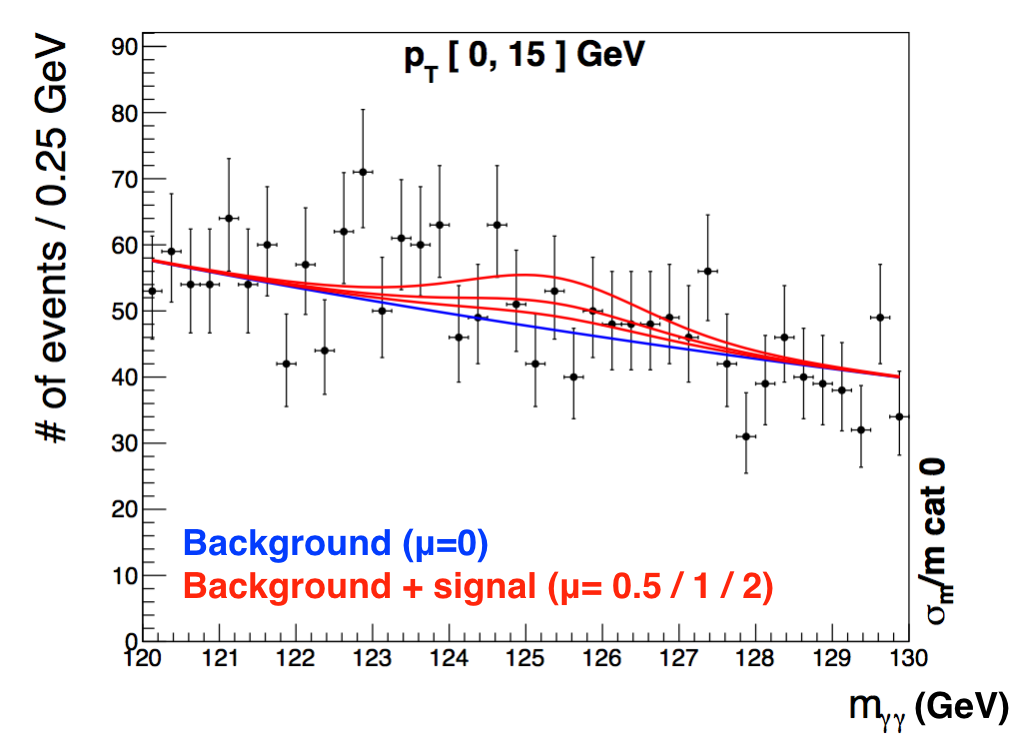
\includegraphics[width=0.49\linewidth]{img/inputs/hgg/example_mgg.png}
    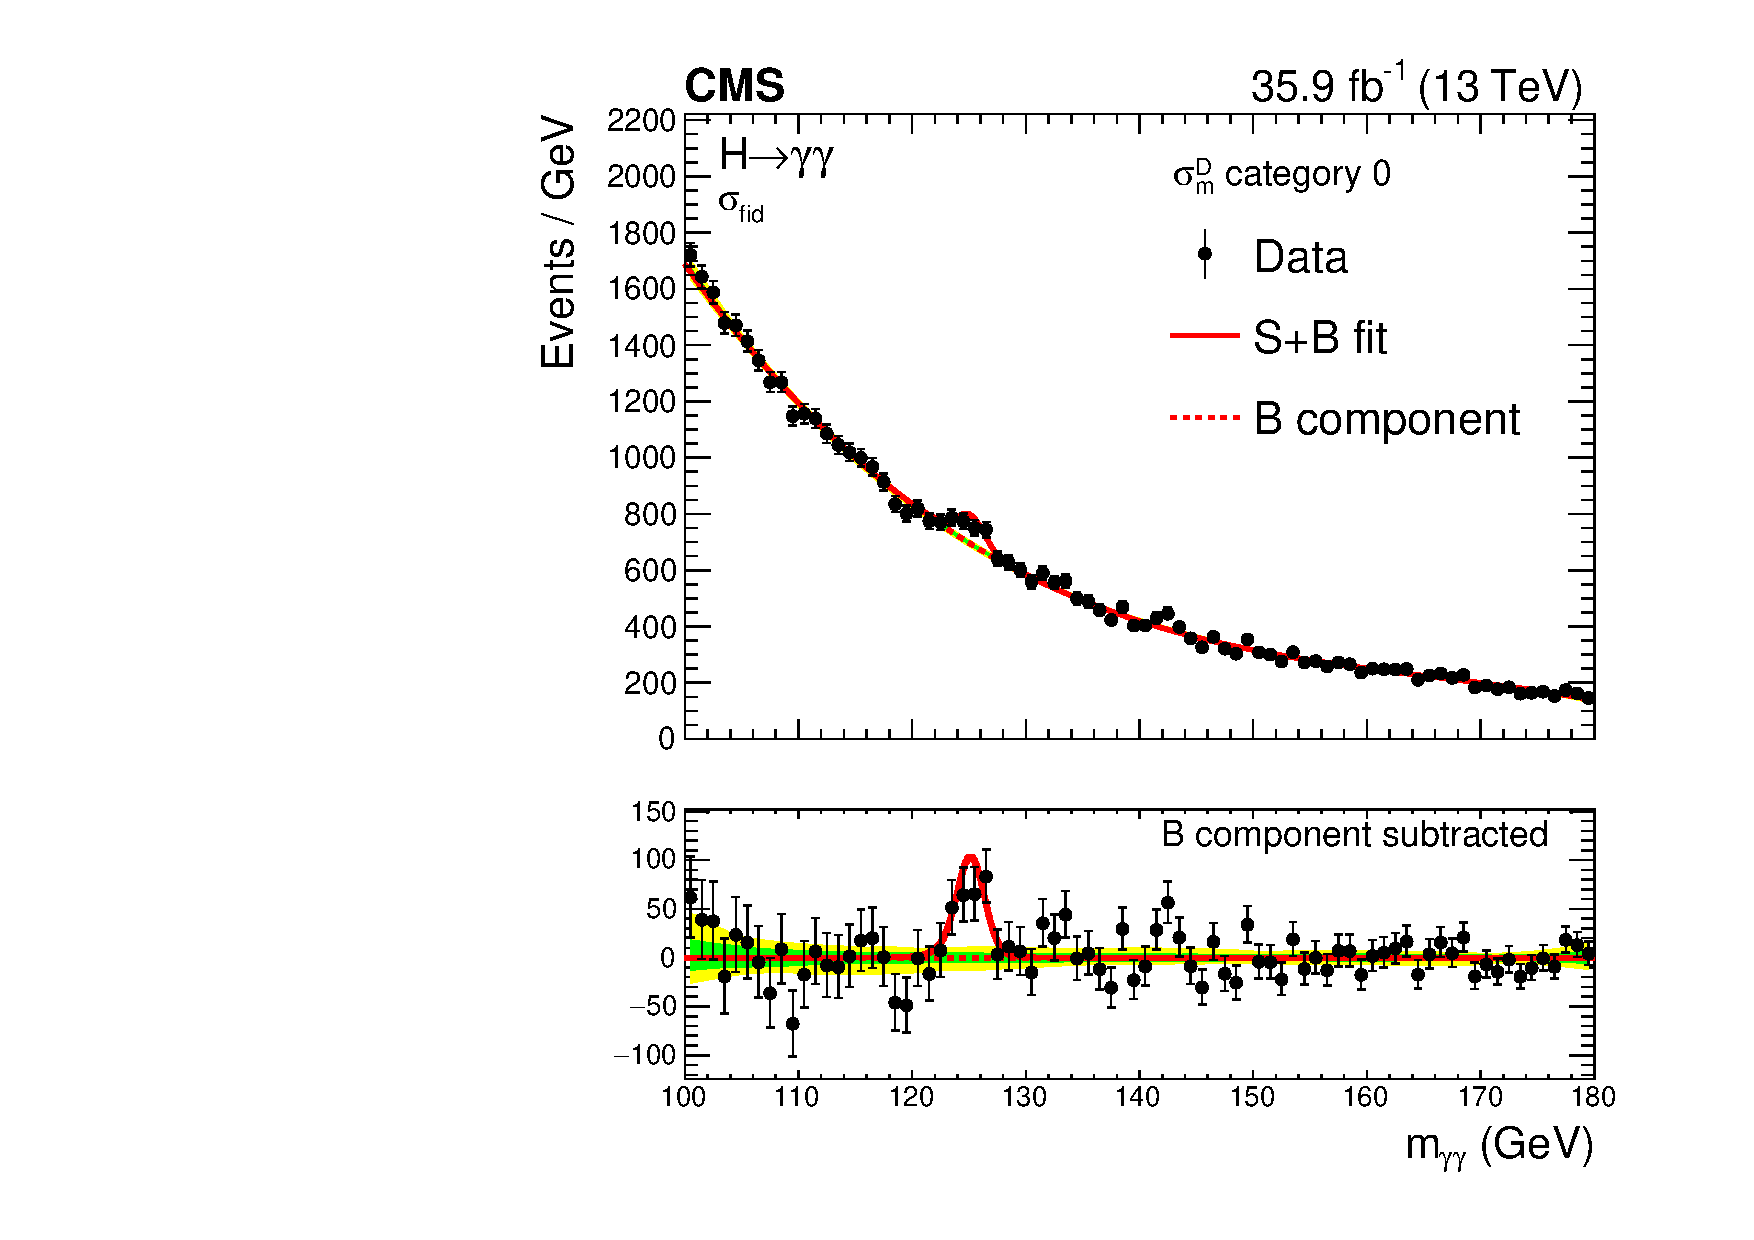
\includegraphics[width=0.49\linewidth]{img/inputs/hgg/example_mgg_allbins.pdf}
    \caption{
        Examples of the $\mgg$ spectrum in the first $\sigma_{\mgg} / \mgg$ category, for only one bin of the $\pth$ spectrum (left) and for all bins combined (right, taken from Ref.~\cite{Sirunyan:2018kta}).
        % 
        In the left plot, the blue line shows an example of a background distribution, the red lines indicate the signal distributions in addition to the background distribution for 0.5, 1.0, and 2.0 times the SM distribution, and the black dots indicate the actual event counts in the 2016 dataset.
        % 
        In the right plot, the red line indicates the combined signal and background fit.
        }
    \label{fig:example_mgg}
  \end{center}
\end{figure}


Because of its comparatively high event count at higher transverse momentum, the $\hgg$ decay channel is the most finely binned one in terms of $\pth$, and is the leading contribution to the overall precision of the combination.
% 
Some of the results obtained in Ref.~\cite{Sirunyan:2018kta} are shown in Fig.~\ref{fig:hgg-results}.


\begin{figure}[hbtp]
  \begin{center}
    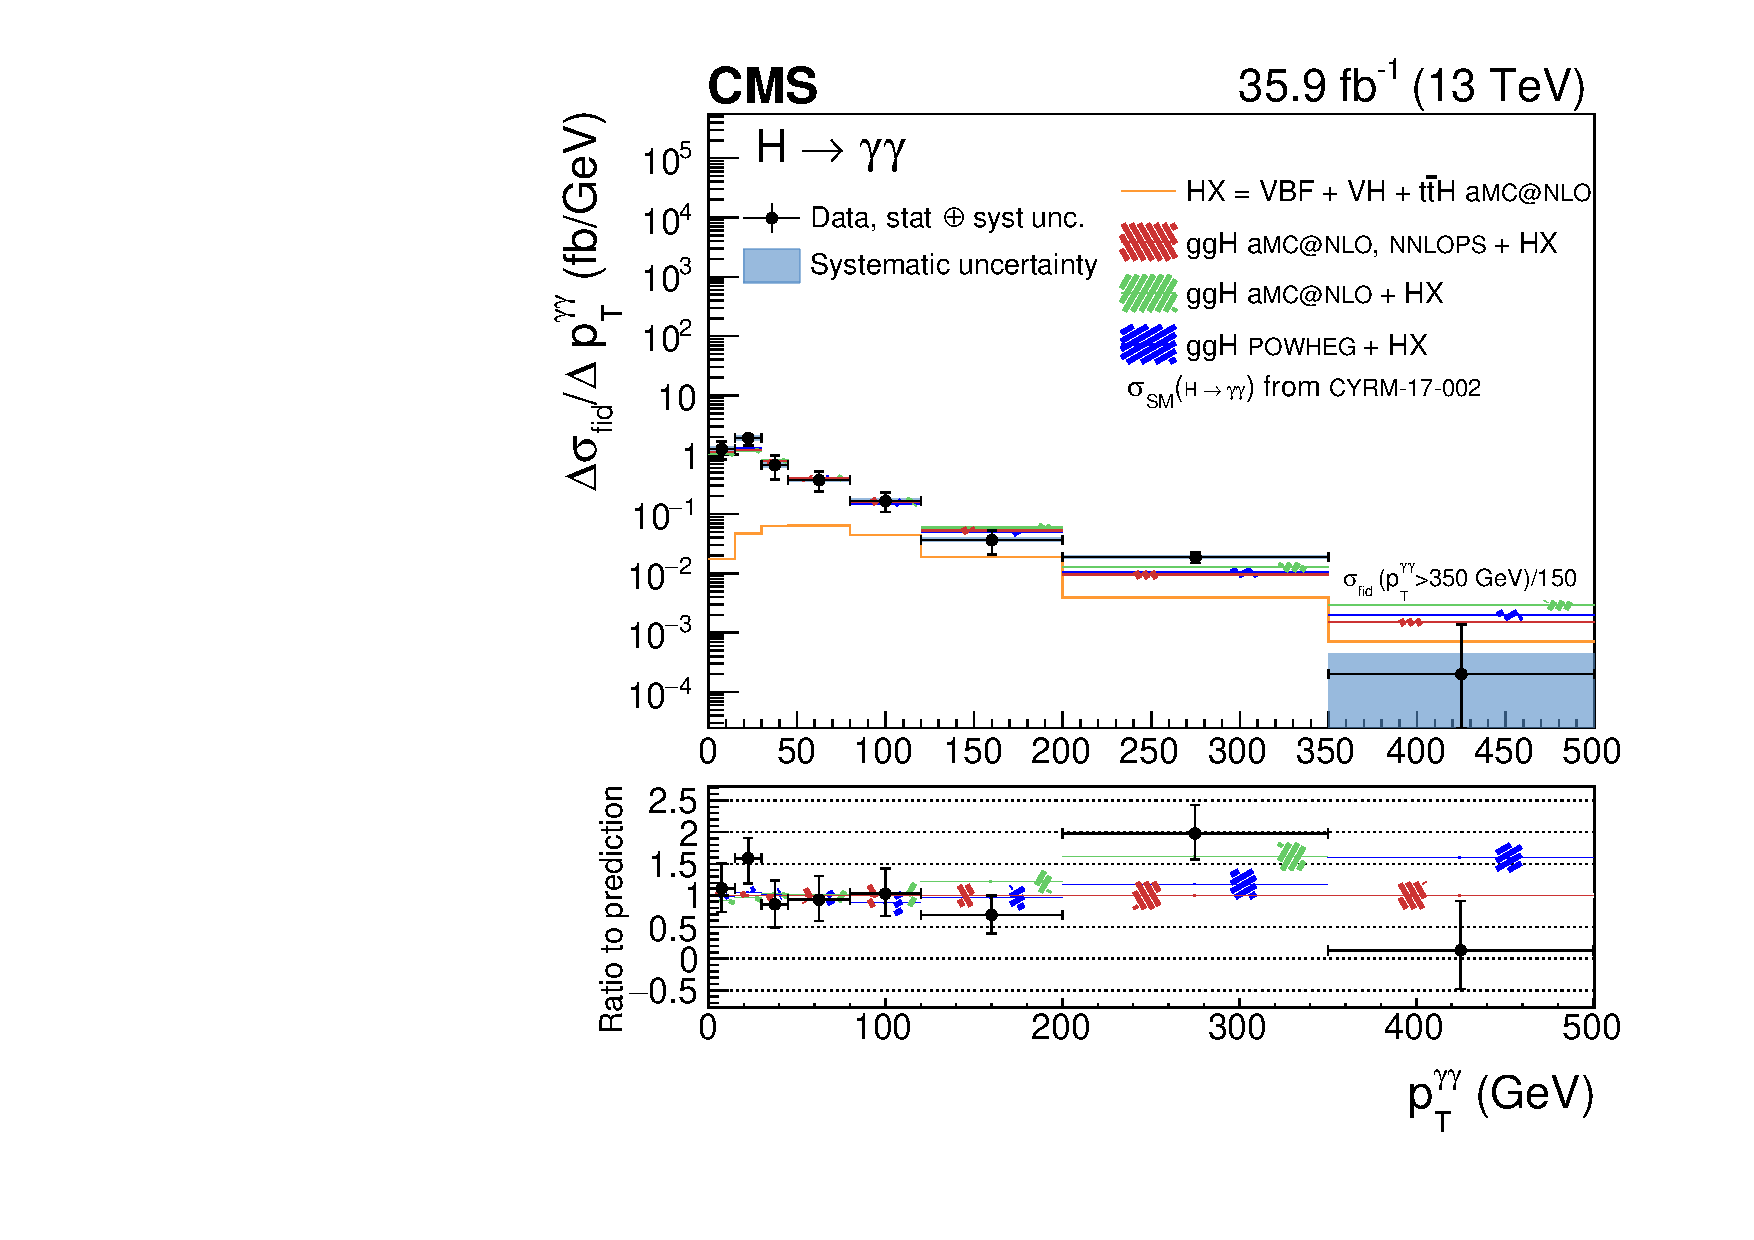
\includegraphics[width=0.49\linewidth]{img/inputs/hgg/pth.pdf}
    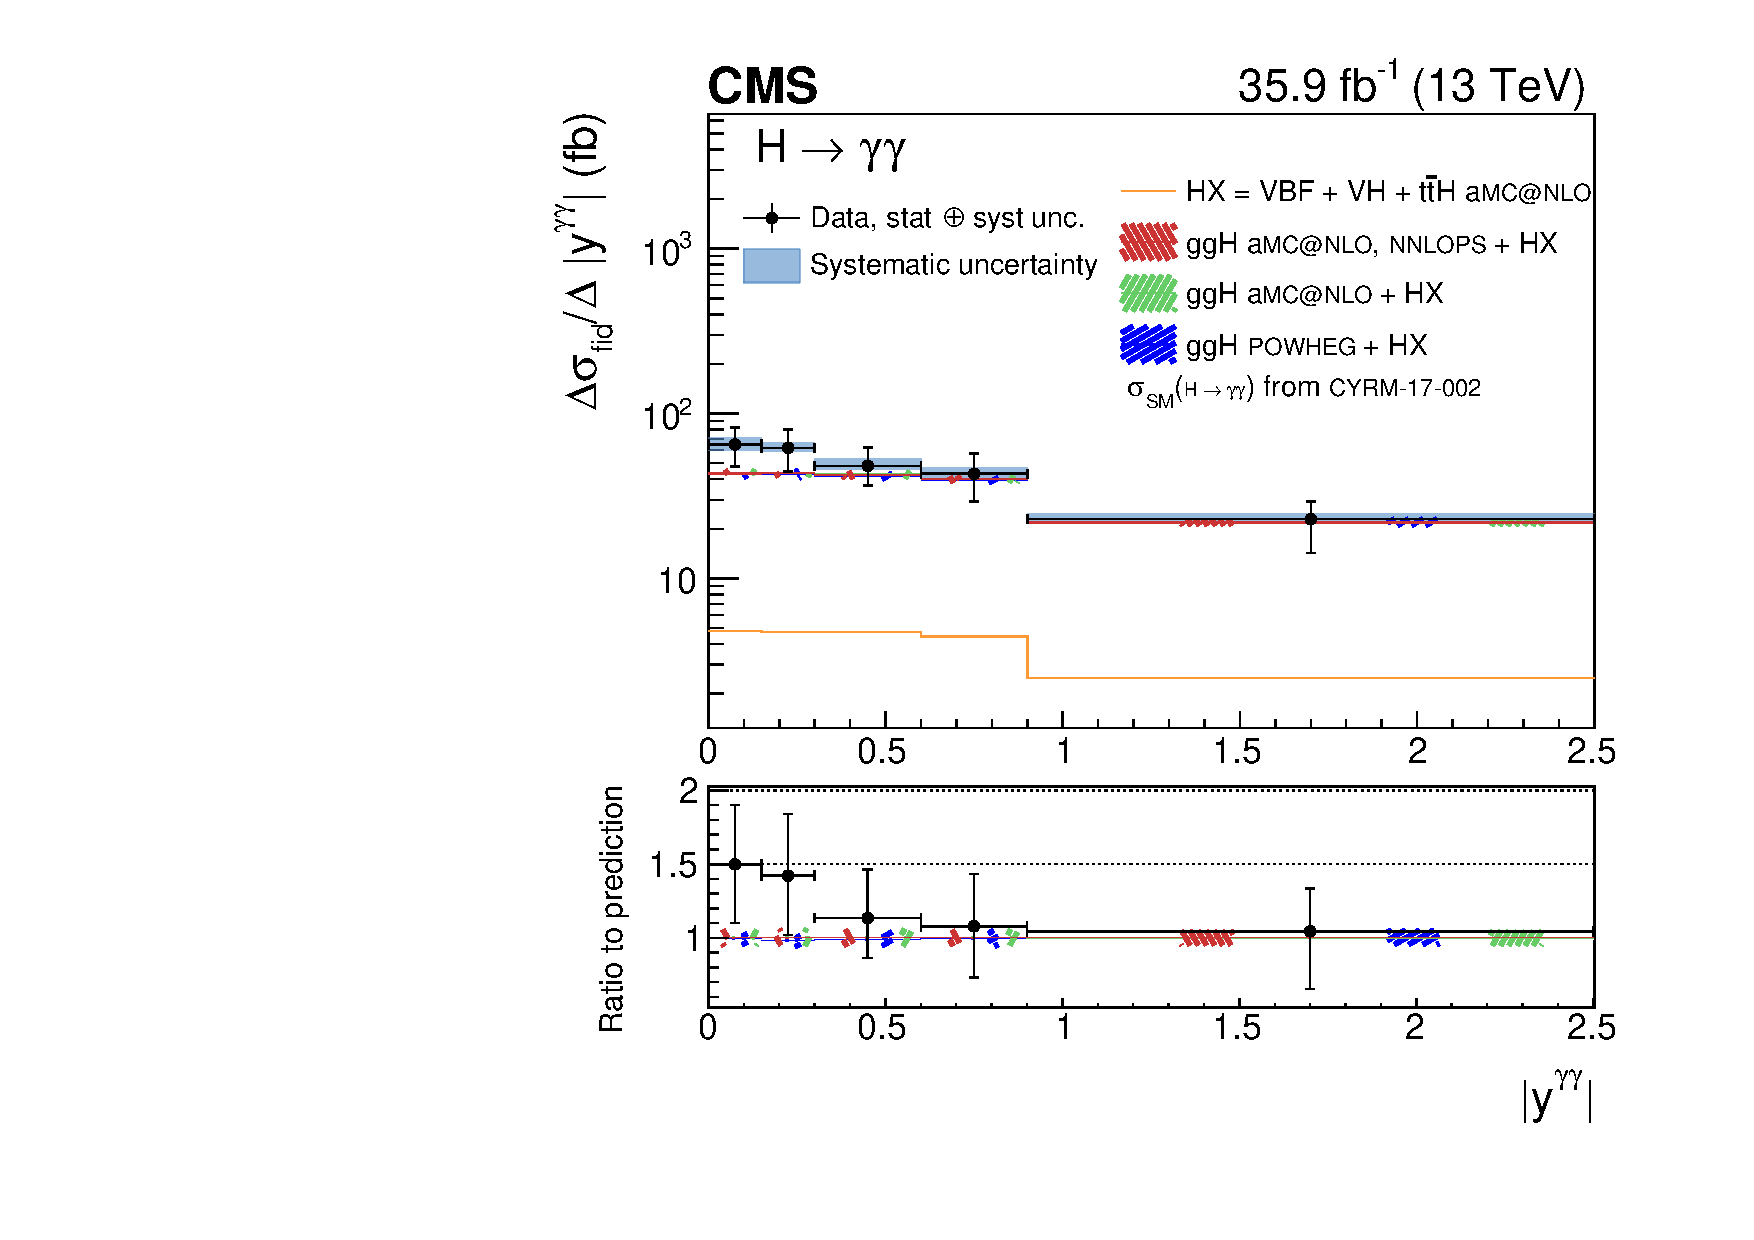
\includegraphics[width=0.49\linewidth]{img/inputs/hgg/absy.pdf}
    \\
    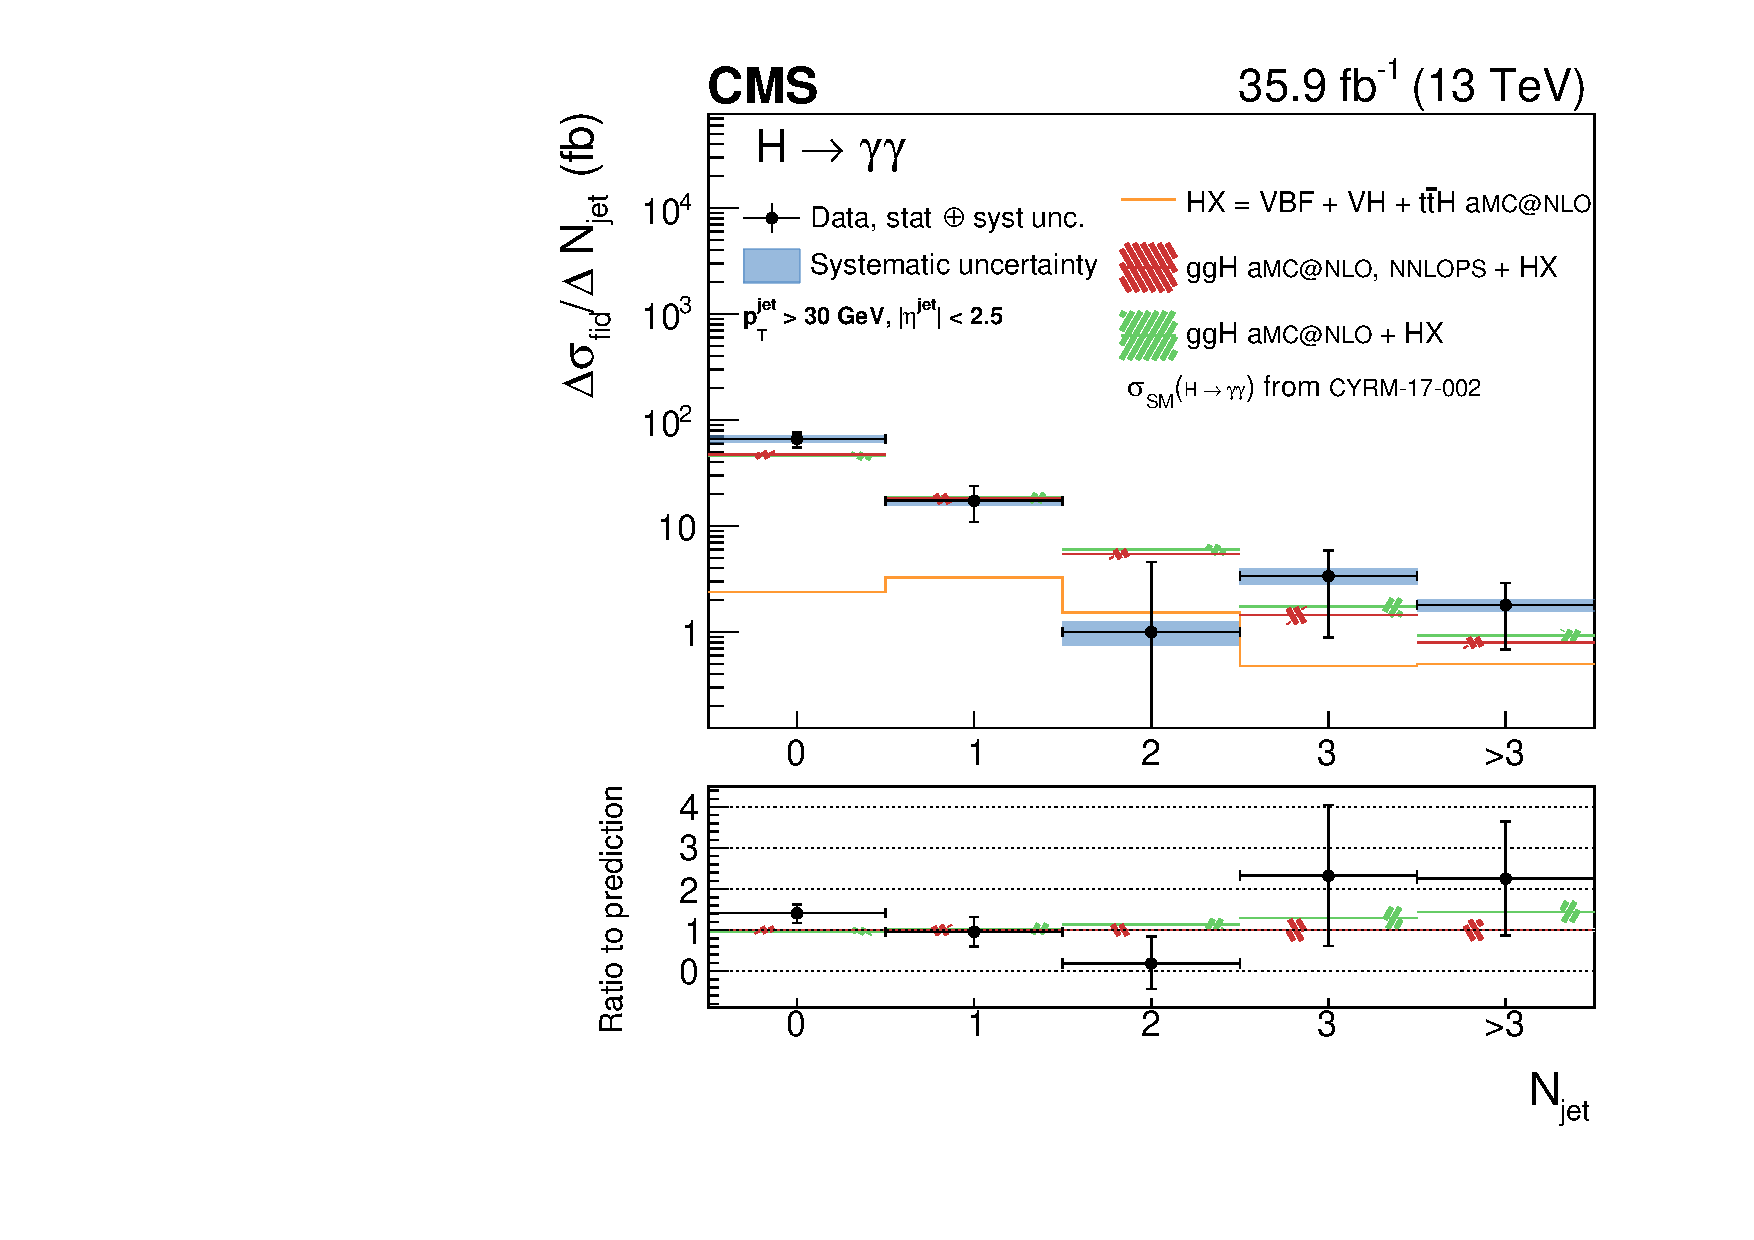
\includegraphics[width=0.49\linewidth]{img/inputs/hgg/njets.pdf}
    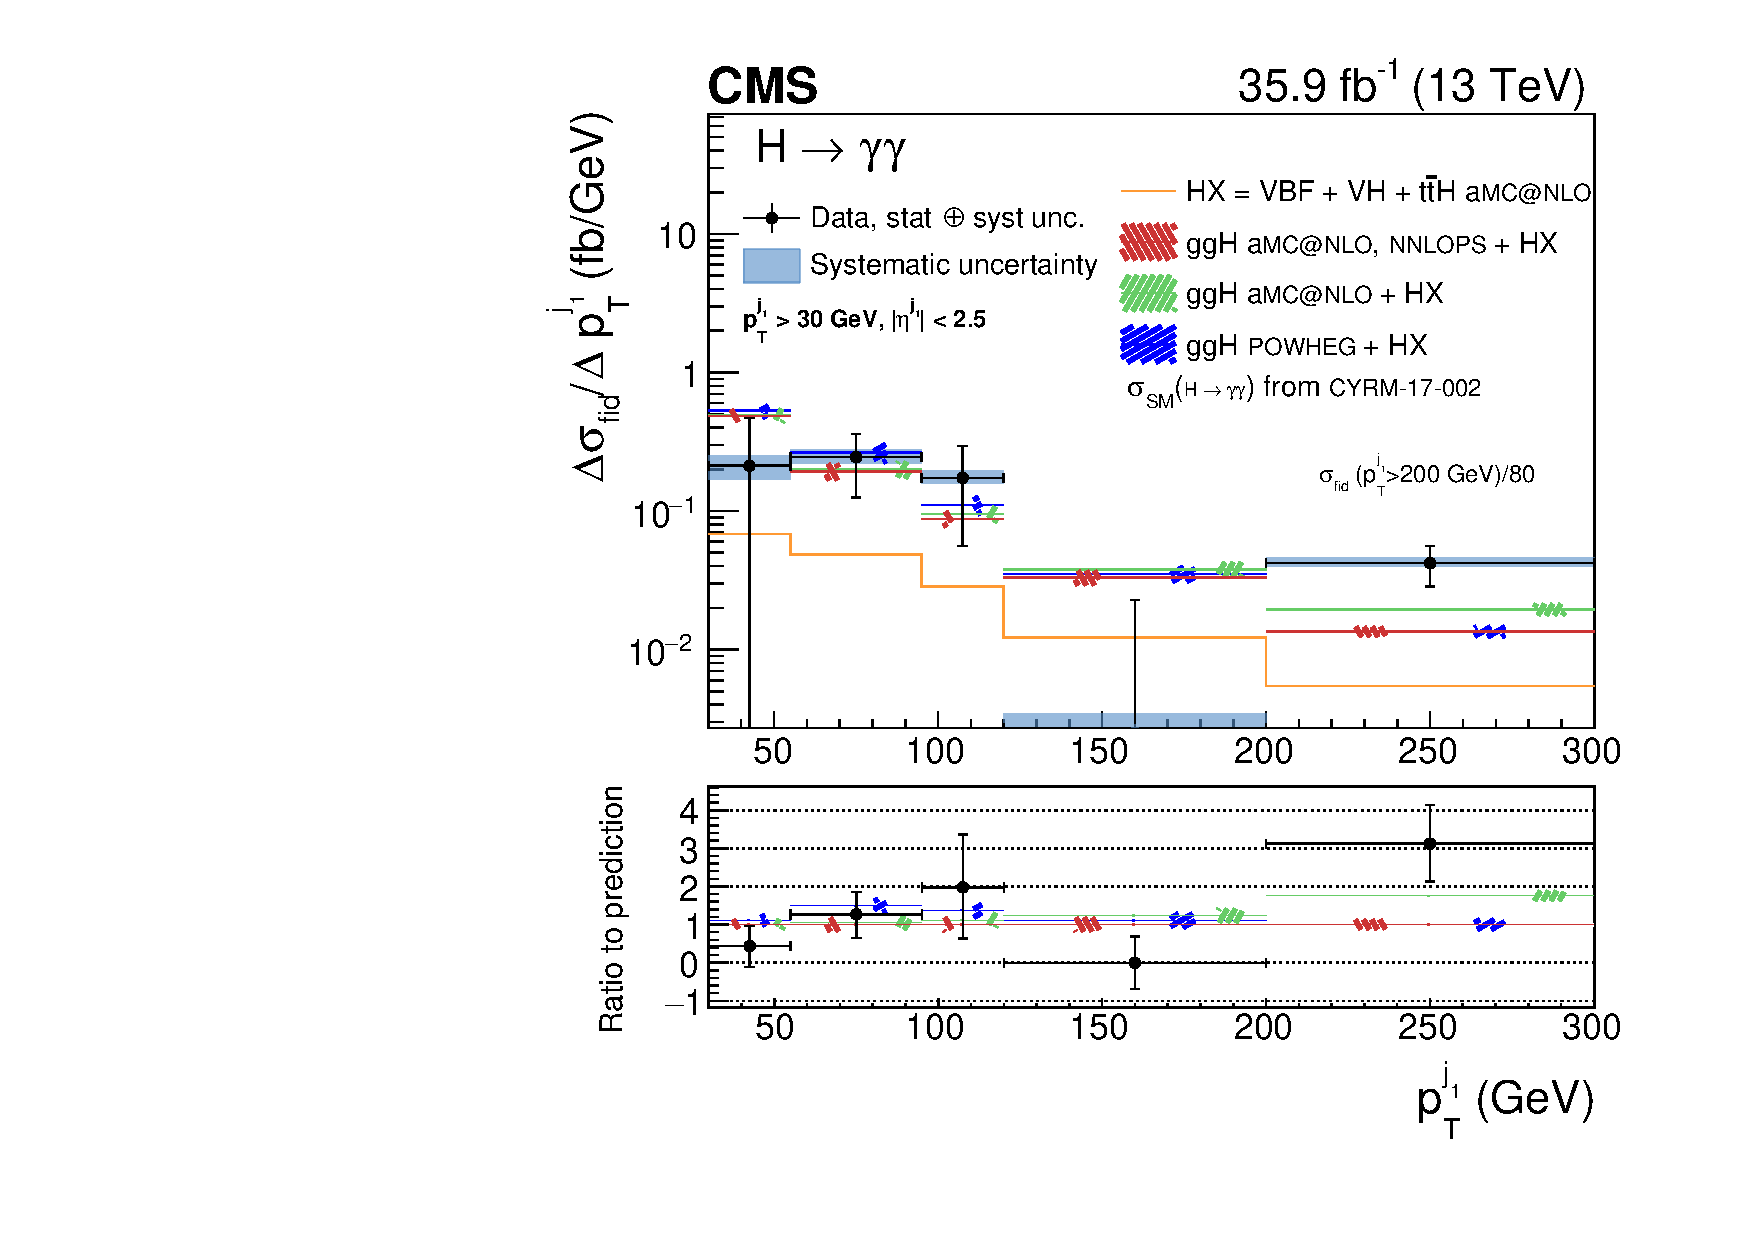
\includegraphics[width=0.49\linewidth]{img/inputs/hgg/ptjet.pdf}
    \caption{
        Differential measurements of the $\pth$ (top left), $\absy$ (top right), $\njets$ (bottom left), and $\ptjet$ (bottom right) spectra from the analysis of the $\hgg$ decay channel.
        % 
        Taken from Ref.~\cite{Sirunyan:2018kta}.
        }
    \label{fig:hgg-results}
  \end{center}
\end{figure}



% ____________________________________________________________________________
\subsection{\texorpdfstring{$\hzztofourl$}{H to ZZ to four leptons}}

\emph{%
Unless otherwise indicated, all information in this section originates from Ref.~\cite{Sirunyan:2017exp}. This section concerns merely a summary of the full analysis; for more details, see the full documentation.
% 
Here the decay channel to four leptons is specifically denoted as `$\hzztofourl$', whereas in the rest of the thesis the notation is simplified to just $\hzz$.
}

Due to the good energy resolution of leptons in the CMS detector, the $\hzztofourl$ decay channel has an exceptionally clean final state, combined with a large signal-to-background ratio.
% 
Its only crutch is the low branching fraction; the first stage of the decay, $\hzz$, has a branching fraction of only $0.26\%$ at $\mh = 125.09\GeV$~\cite{deFlorian:2016spz}; combined with the second stage, requiring the decays of the $\zboson$ bosons to either electrons or muons, reduces the branching fraction further to $1.251 \times 10^{-2}$ \%~\cite{deFlorian:2016spz}.
% 
Despite its low branching fraction, the differential measurements performed in the $\hzz$ decay channel have a good precision at low $\pt$; at higher $\pt$ the event count becomes very small and the precision deteriorates.


The analysis strategy concerns a fit to the four-lepton mass $\mfourl$ spectrum, in which the signal presents itself as a narrow peak on top of a small continuum background.
% 
The background contains an irreducible contribution originating from direct $\zboson\zboson$ production, and a reducible contribution with misidentified leptons.
% 
The main reducible backgrounds concerns $\zboson + \bbbar$ and $\ttbar$, where the quarks decay leptonically, and $\zboson + \text{jets}$ events where the jets are misidentified as leptons.
% 
The $\mfourl$ spectrum, including the obtained event counts, is shown in Fig.~\ref{fig:example_mfourl}.


In order to reduce the contamination from muons originating from in-flight decays, the selected leptons are required to have the same primary vertex.
% 
To achieve this, the ratio of the impact parameter, describing to what extent the tracks of the leptons line up with the primary vertex, over the uncertainty on the impact parameter is required to be less than 4.
% 
To further reduce the misidentified lepton rate, cuts are also placed on the isolation with respect to hadronic and photonic activity.


Also the analysis in the $\hzztofourl$ decay channel employs a fiducial phase space definition.
% 
From the four reconstructed leptons, two leptons are required to have $\pt > 10\GeV$, and at least one must have $\pt > 20\GeV$.
% 
All leptons are also required to separated in angular space by at least $\Delta R > 0.02$.
% 
On a higher level, the leading reconstructed $\zboson$ boson candidate must have an invariant mass of at least 40\GeV, and $\mfourl > 70\GeV$.
% 
The event categorization follows simply the lepton configuration in the final state: 4 electrons, 4 muons, or 2 electrons and 2 muons.


Due to its poor branching fraction, the event counts for the $\hzztofourl$ channel in the higher $\pth$ bins is very small, and the binning is chosen to be coarser than in the case of the $\hgg$ decay channel.
% 
The differential measurements are shown in Fig.\ref{fig:hzz-results} for the $\pth$, $\njets$, and $\ptjet$ spectra.



\begin{figure}[hbtp]
  \begin{center}
    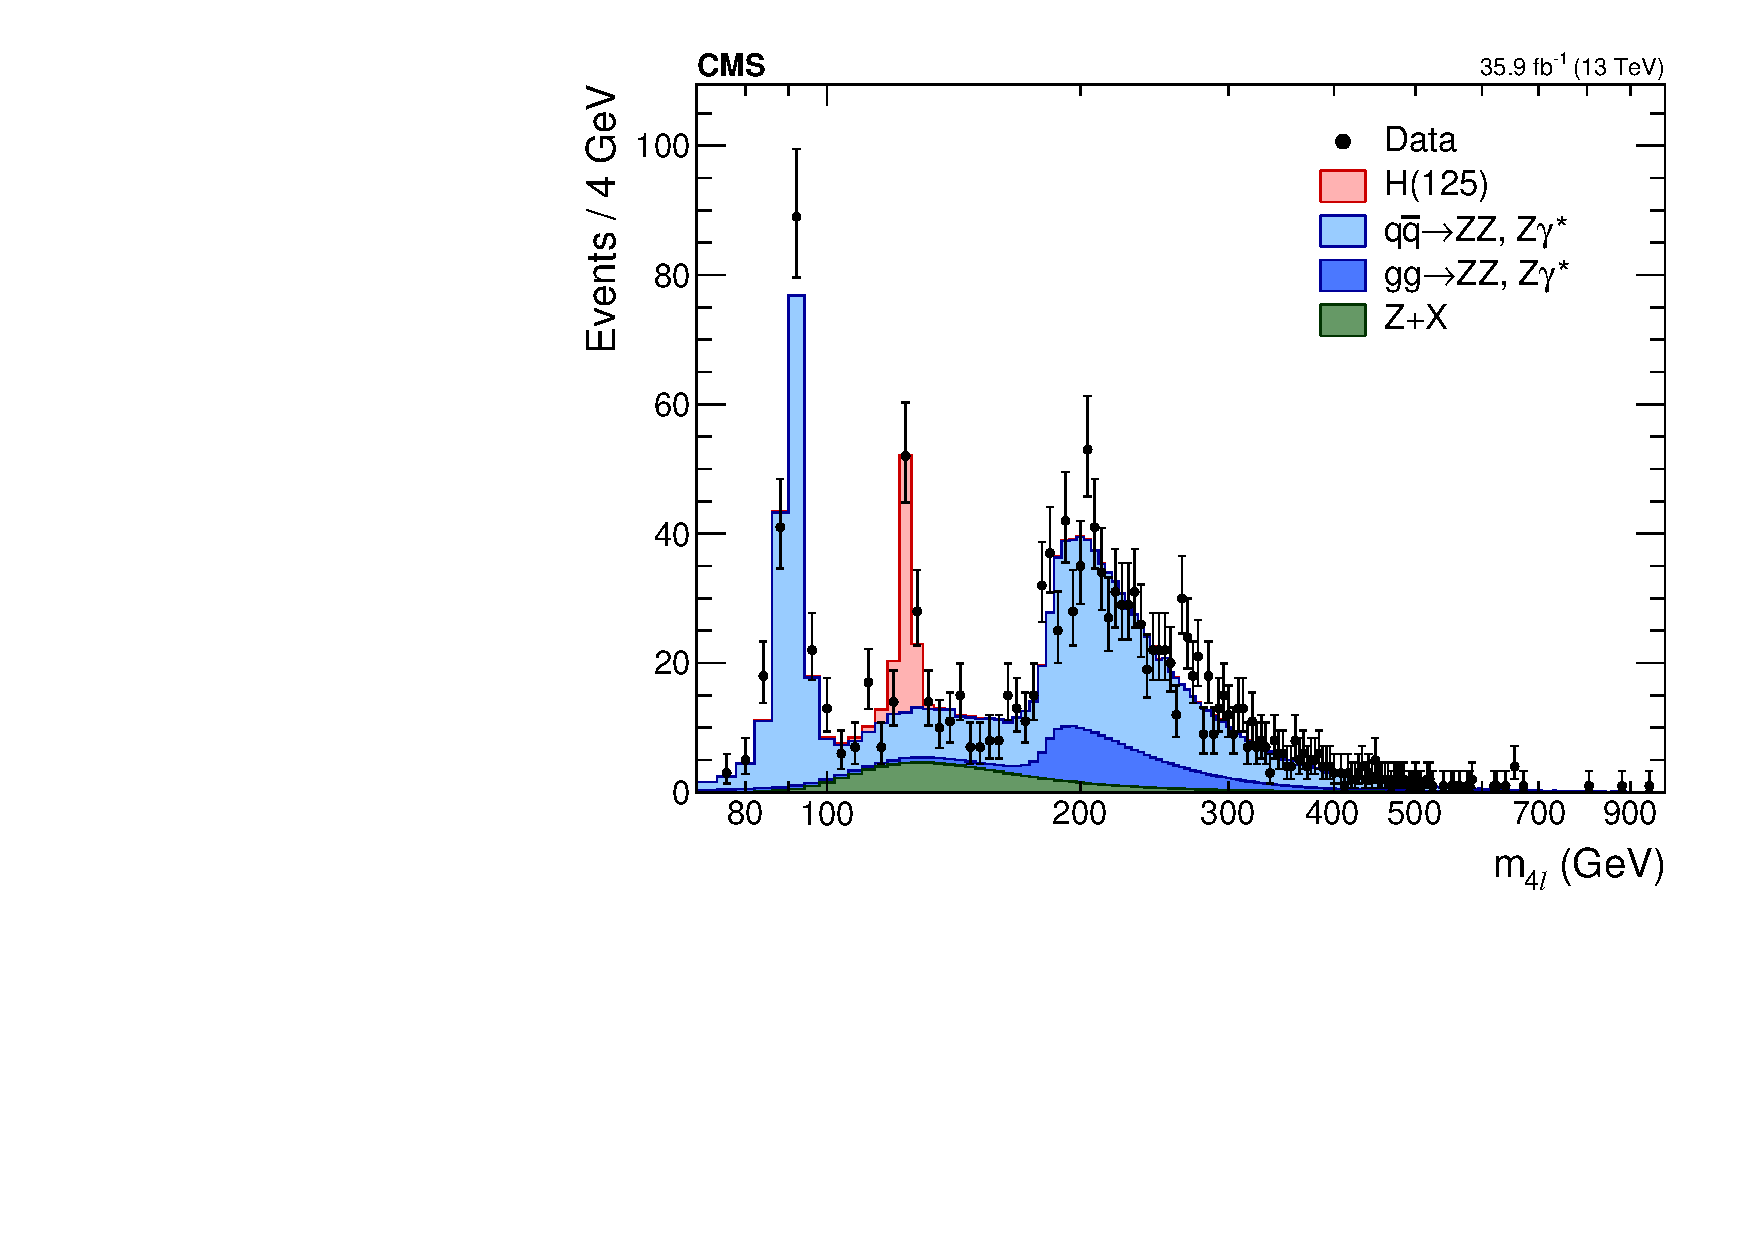
\includegraphics[width=0.7\linewidth]{img/inputs/hzz/m4lspectrum.pdf}
    \caption{
        Example of the $\mfourl$ spectrum.
        % 
        The color-shaded area indicate the expected event counts according to the SM and the black dots indicate the actual event counts in the 2016 dataset.
        }
    \label{fig:example_mfourl}
  \end{center}
\end{figure}

\begin{figure}[hbtp]
  \begin{center}
    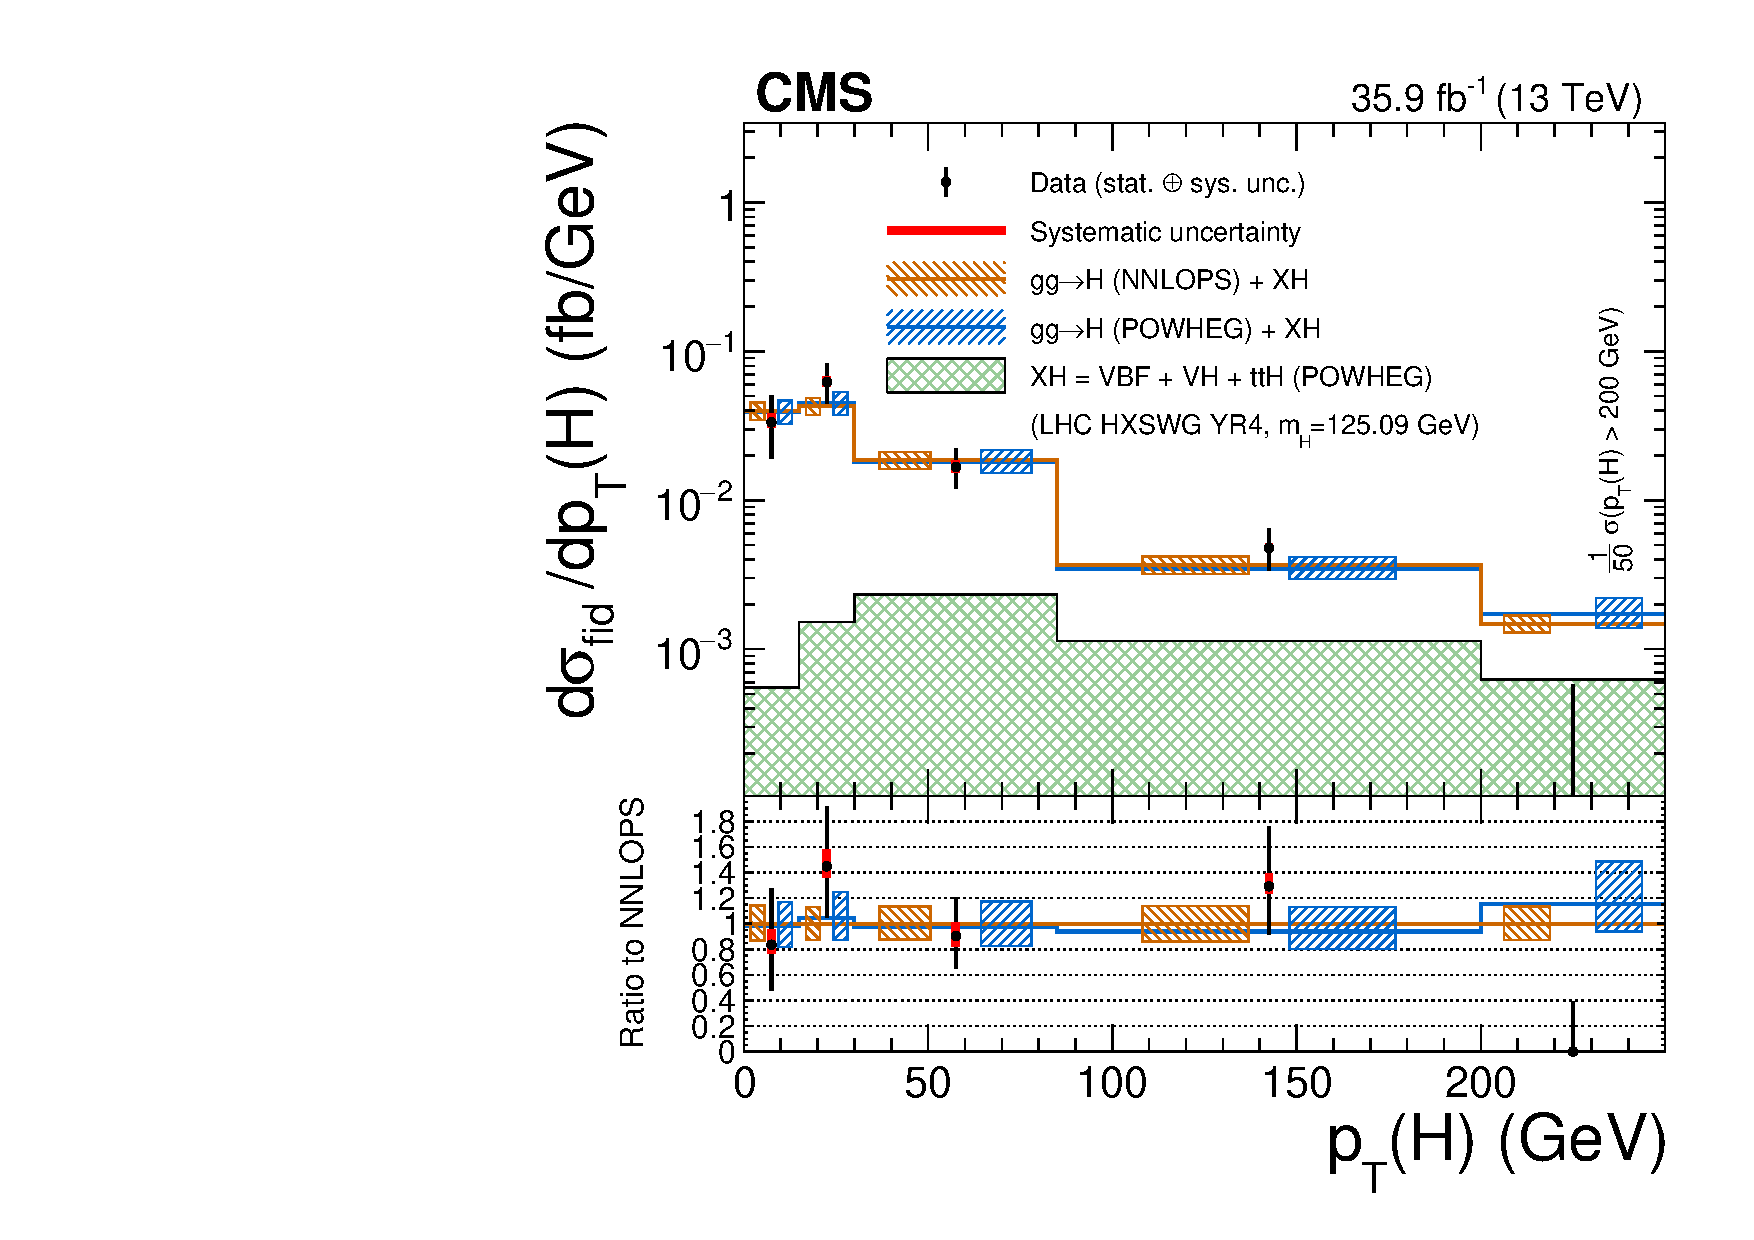
\includegraphics[width=0.49\linewidth]{img/inputs/hzz/pth.pdf}
    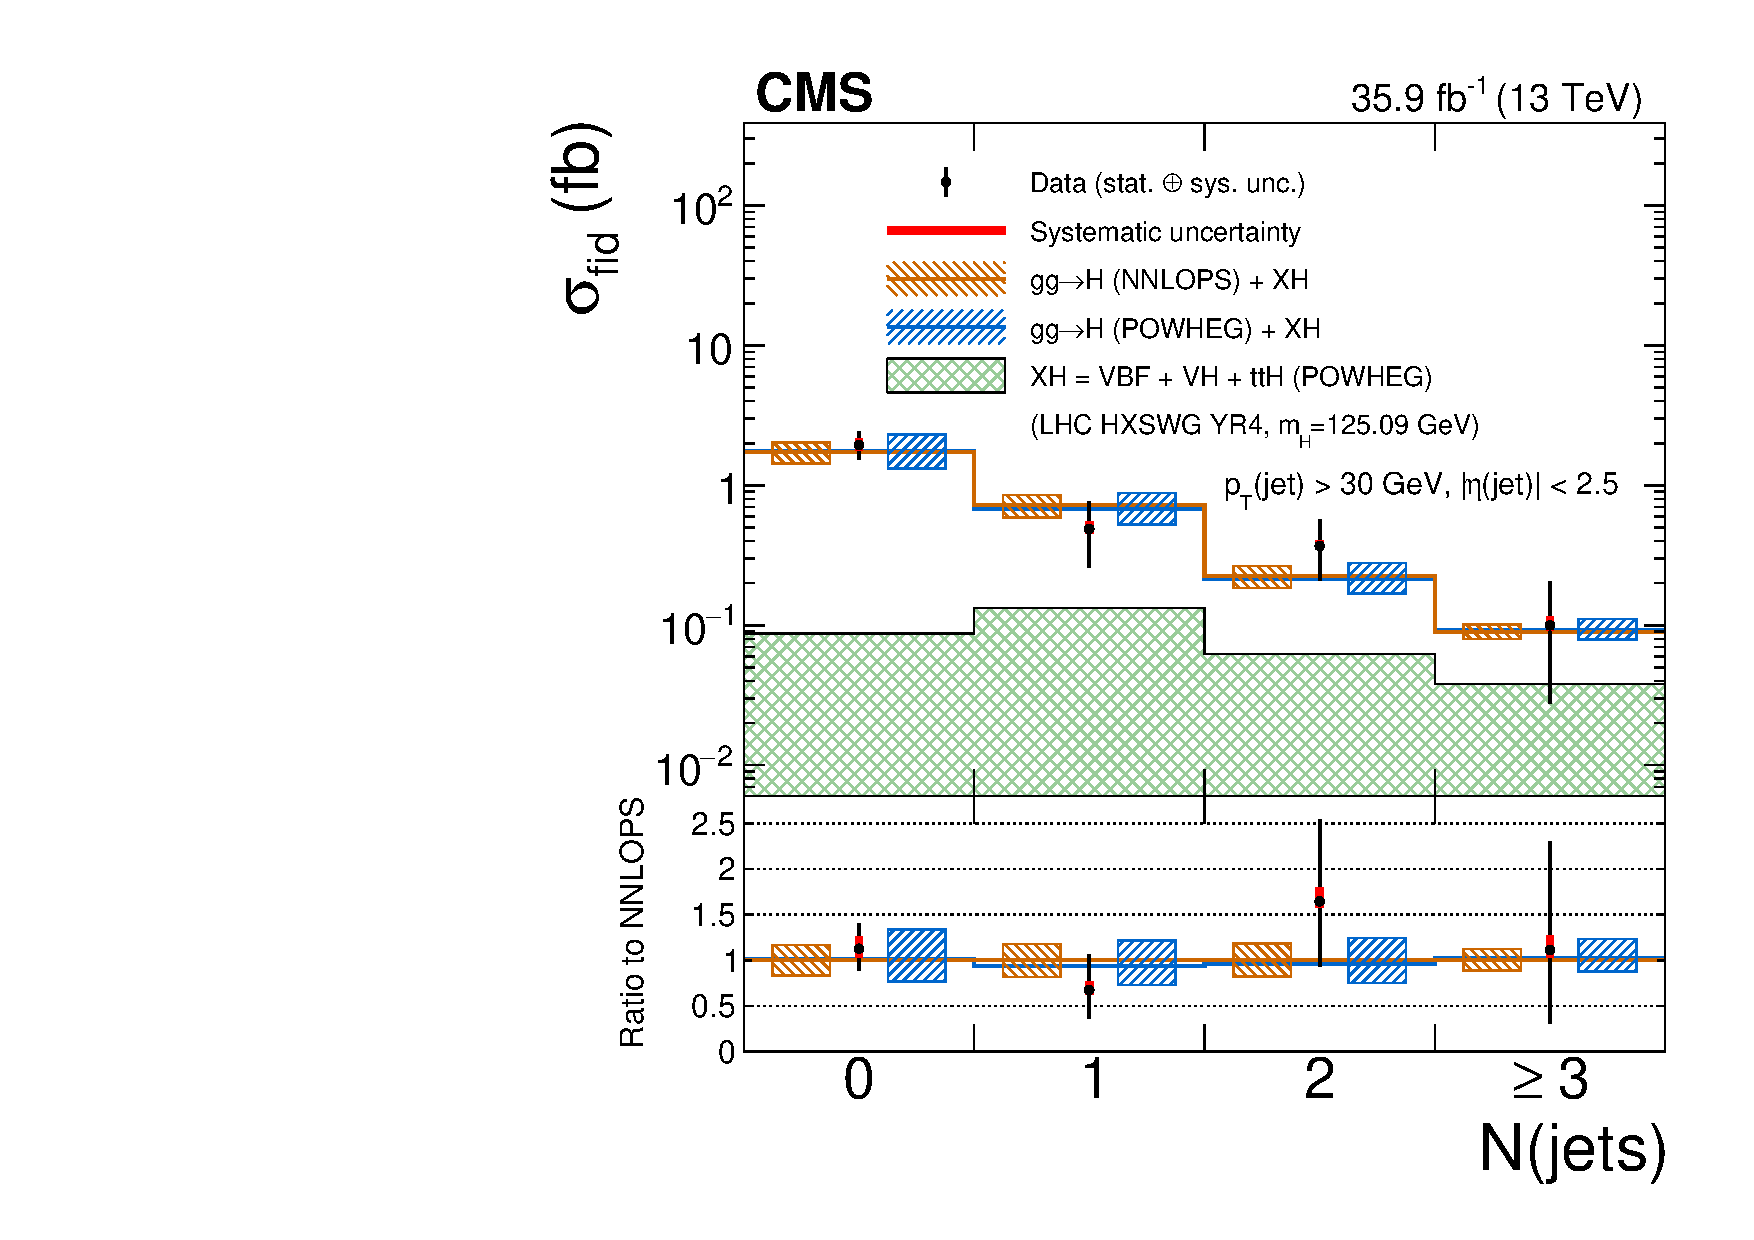
\includegraphics[width=0.49\linewidth]{img/inputs/hzz/njets.pdf}
    \\
    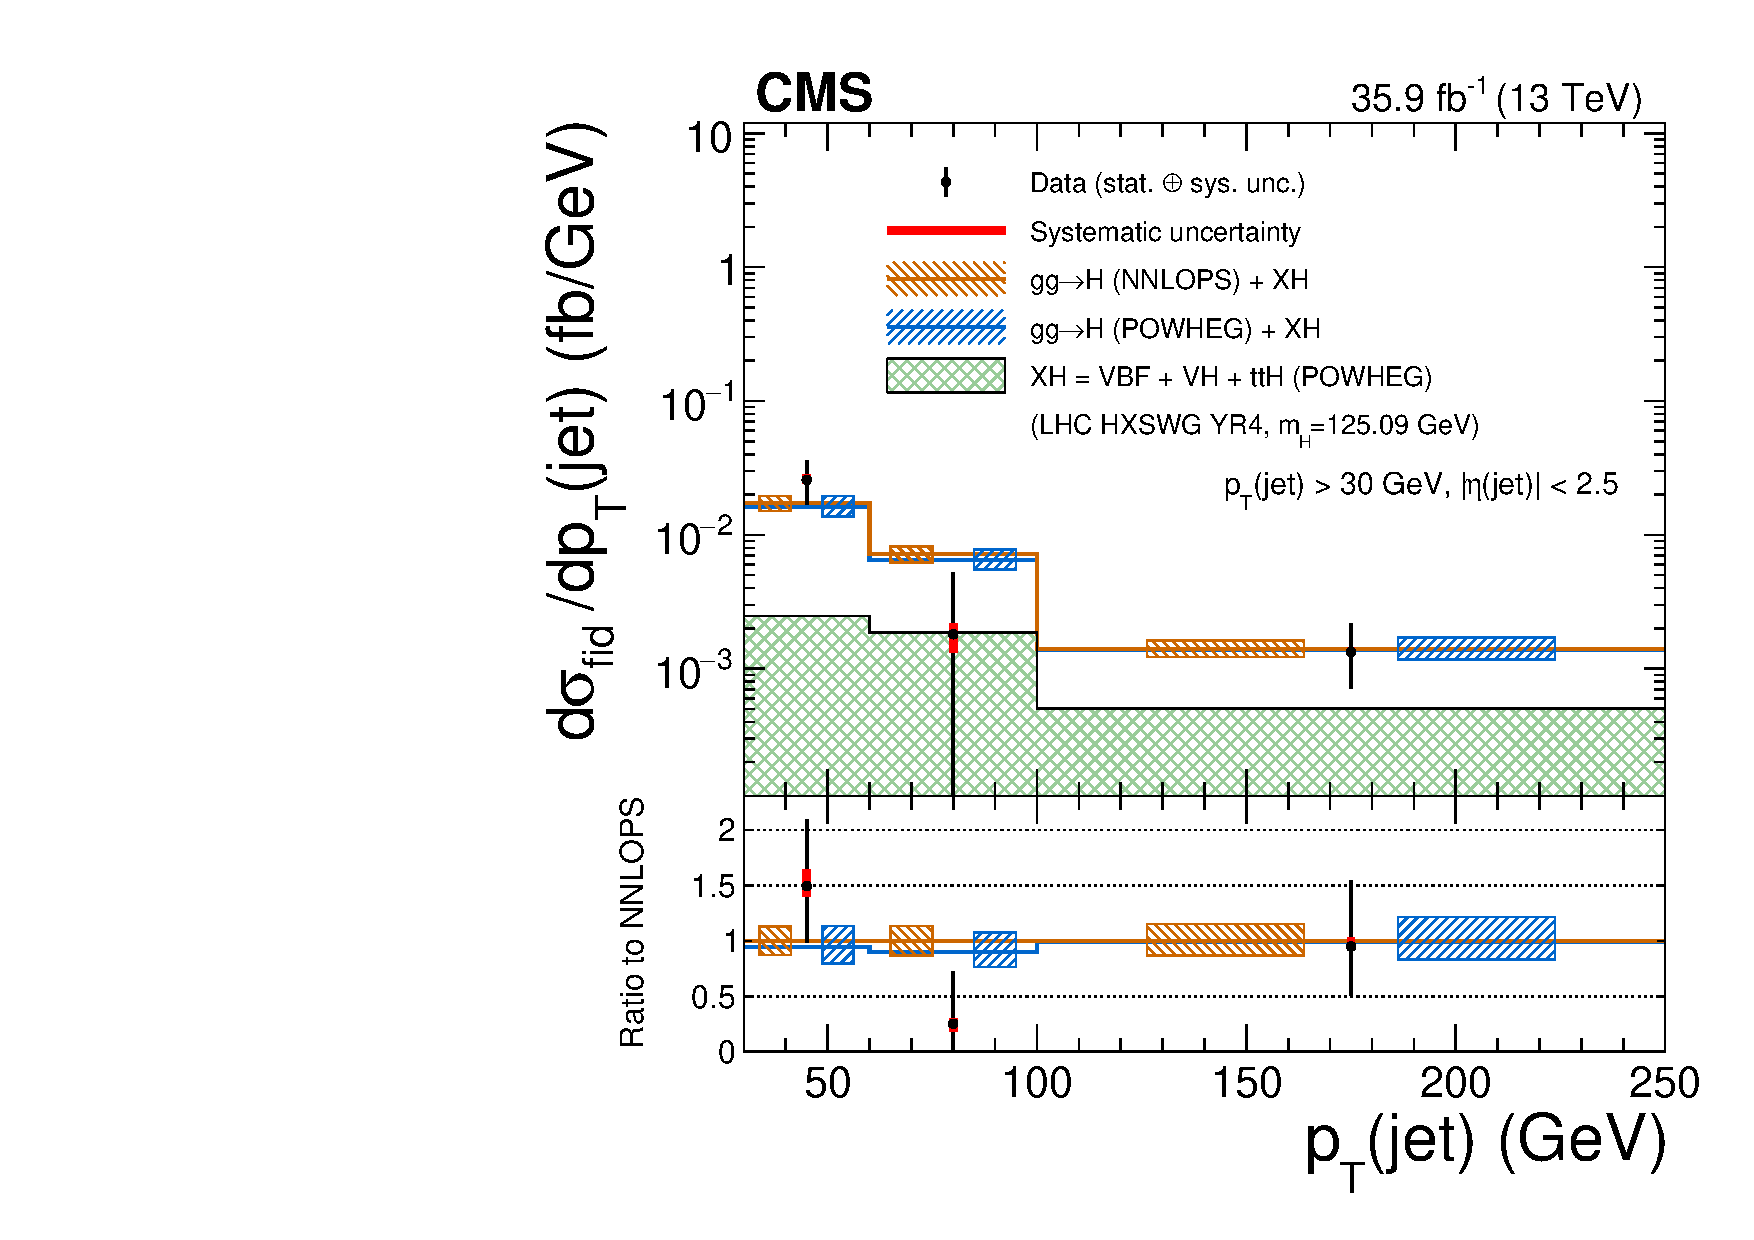
\includegraphics[width=0.49\linewidth]{img/inputs/hzz/ptjet.pdf}
    \caption{
        Differential measurements of the $\pth$ (top left), $\njets$ (top right), and $\ptjet$ (bottom) spectra from the analysis of the $\hzztofourl$ decay channel.
        % 
        Taken from Ref.~\cite{Sirunyan:2017exp}.
        }
    \label{fig:hzz-results}
  \end{center}
\end{figure}



% ____________________________________________________________________________
\subsection{\texorpdfstring{Boosted $\ggh\to\bbbar$}{Boosted ggHbb}}

\emph{%
Unless otherwise indicated, all information in this section originates from Ref.~\cite{Sirunyan:2017dgc}. This section concerns merely a summary of the full analysis; for more details, see the full documentation.
}

The final input concerns the search for a highly boosted (i.e. large transverse momentum) Higgs boson decaying to two bottom quarks.
% 
For a Higgs boson with a large transverse momentum, the two resulting bottom quarks become very collimated, are are reconstructed in the detector as a single `fat' jet.
% 
The challenge in this analysis is to retrieve the decay products via close inspection of the internal substructure of the fat jet.
% 
As the Higgs mass is close to the $\zboson$ boson mass, contamination with $\zboson\to\bbbar$ decays is unavoidable.
% 
The $\zboson\to\bbbar$ decays are used to validate the analysis, and its signal strength is fitted in tandem with the one for the Higgs decay channel.


In terms of event selection, the analysis requires, clearly, the presence of a single fat jet, defined as an anti-$\kt$ jet~\cite{Cacciari:2008gp} with a distance parameter of $0.8$, $\pt > 450$\GeV, and $\abs{\eta}<2.5$.
% 
To reduce the background from other electroweak processes, events with isolated electrons, muons or $\taulepton$ leptons with $\pt > 10$, $10$, and $18\GeV$, respectively, are vetoed.
% 
Also events with a very large amount of missing transverse energy are vetoed, as this is in principle not expected for this analysis.
% 
The fat jet is ran through the soft-drop algorithm~\cite{Dasgupta:2013ihk,Larkoski:2014wba}: Taking the reverse order of the anti-$\kt$ clustering, the algorithm continually removes the softer constituent as long as
% 
\begin{linenomath*}
\begin{equation}
\frac{ \text{min}( \pt^1, \pt^2 ) }{ \pt^1 + \pt^2 }
    \leq
    z \left( \frac{\Delta R_{12}}{R_0} \right)^\beta
\,,
\end{equation}
\end{linenomath*}
% 
where $\pt^1$ and $\pt^2$ are the transverse momenta of the unclustered components, $\Delta R_{12}$ is their distance in angular space, $R_0$ is the radius of the initial fat jet, and $z$ and $\beta$ are parameters of the algorithm.
% 
The algorithm is designed to remove soft and wide-angle radiation.
% 
In the $\hbb$ analysis, the parameters $z$ and $\beta$ are chosen to be $0.1$ and $0$, respectively.
% 
The soft-drop algorithm reduces the mass of the fat jet to the new mass $\msd$, also called the soft-drop mass; for events in which the fat jet originates from the QCD background, the mass drop is very large, whereas for fat jets originating from the signal, the mass drop is less pronounced.
% 
For signal events, $\msd$ is close to the mass of the Higgs boson.
% 
To avoid finite-cone effects and the nonperturbative regime of the $\msd$ calculation, an additional selection is applied based on the dimensionless mass scale variable for QCD jets $\rho=\log\left(\msd^2/\pt^2\right)$~\cite{Dasgupta:2013ihk}, which relates the fat jet $\pt$ to the fat jet mass.


An excellent discriminator for signal fat jets and fat jets originating from the QCD background is the $N^1_2$ variable, which is computed using the ratio of the 2-point and 3-point generalized energy correlation functions~\cite{Larkoski:2013eya}.
% 
It measures to what extent a jet is consistent with having a two-prong substructure.
% 
After a transformation to reduce the correlation of $N^1_2$ with $\rho$ and $\pt$, $N^1_2 \to N_2^{1,\text{DDT}}$ (where DDT stands for Designed Decorrelated Tagger~\cite{Dolen:2016kst}), a selection $N_2^{1,\text{DDT}} < 0$ is applied.


The double-$\bquark$-tagger algorithm~\cite{Sirunyan:2017ezt}, based on input variables related to substructure and observables optimized for $\bquark$ identification, is applied on the selected events.
% 
Tagged fat jets are tagged such that the fat jets originating from the QCD background are misidentified in $1\%$ of the cases, and with a $33\%$ efficiency for the signal fat jets.
% 
Events with a double-$\bquark$-tagged fat jet then constitute the so-called `passing' region, whereas those without it constitute the `failing' region.
% 
The failing region is used to constrain the QCD background.
% 
The ratio of passing over failing events $R_\text{p/f}$ as a function of $\msd$ and $\pt$ is almost flat; the small remaining dependence on $\msd$ and $\pt$ is parametrized using a polynomial, where the order of the polynomial is determined by a Fisher $F$-test.
% 
Much like in the previous two decay channels, the signal is extracted based on a fit to the $\msd$ spectra, where the categories correspond to the passing and failing regions, and to six bins of reconstructed $\pt$ (within $450 < \pt < 1000\GeV$).
% 
The analysis employs no fiducial phase space.


The $\msd$ spectrum in the passing region is shown in Fig.~\ref{fig:hbbresults} (left).
% 
The peak from $\zboson\to\bbbar$ is clearly visible, and is in fact observed with a significance of $5.1$ standard deviations.
% 
Figure~\ref{fig:hbbresults} (right) shows the fit of the $\zboson\to\bbbar$ and $\hbb$ channels.


\begin{figure}[hbtp]
  \begin{center}
    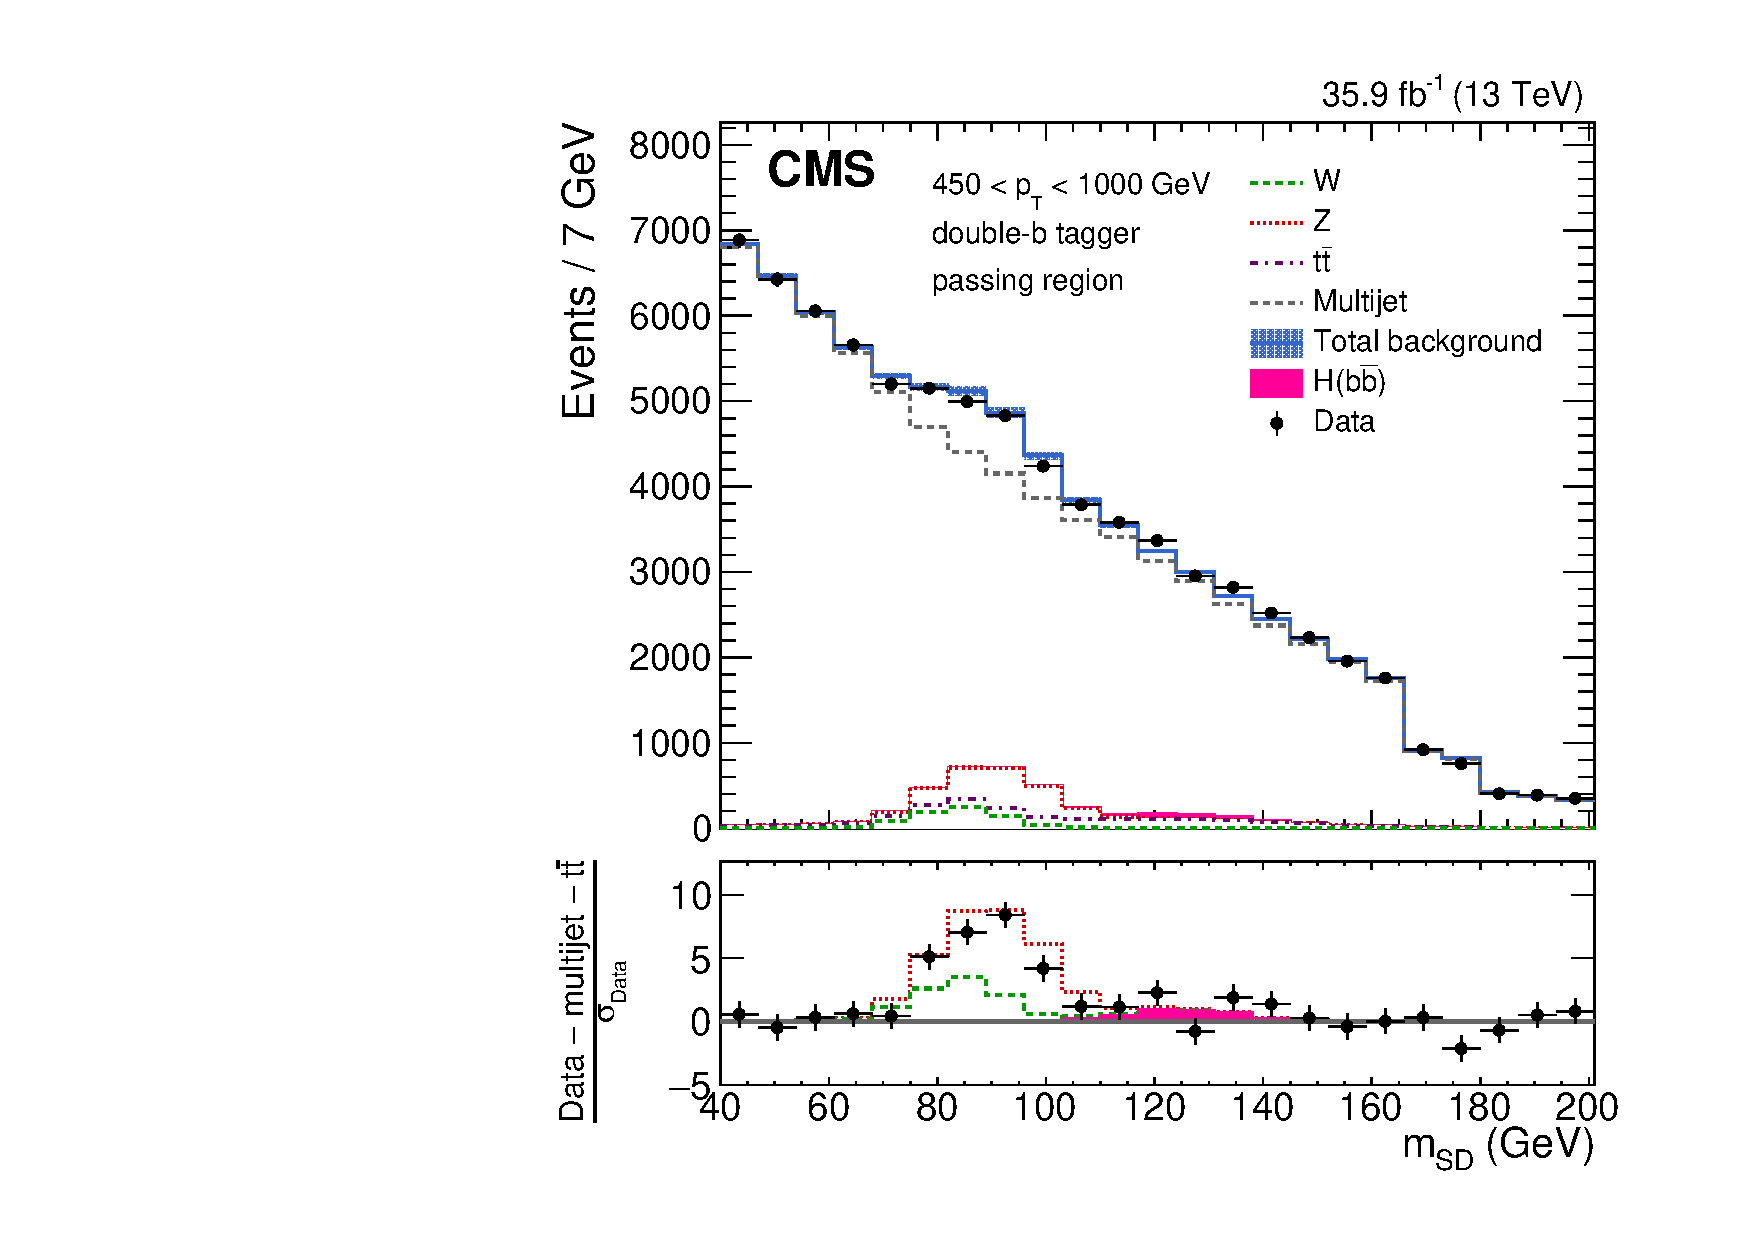
\includegraphics[width=0.49\linewidth]{img/inputs/hbb/msd.pdf}
    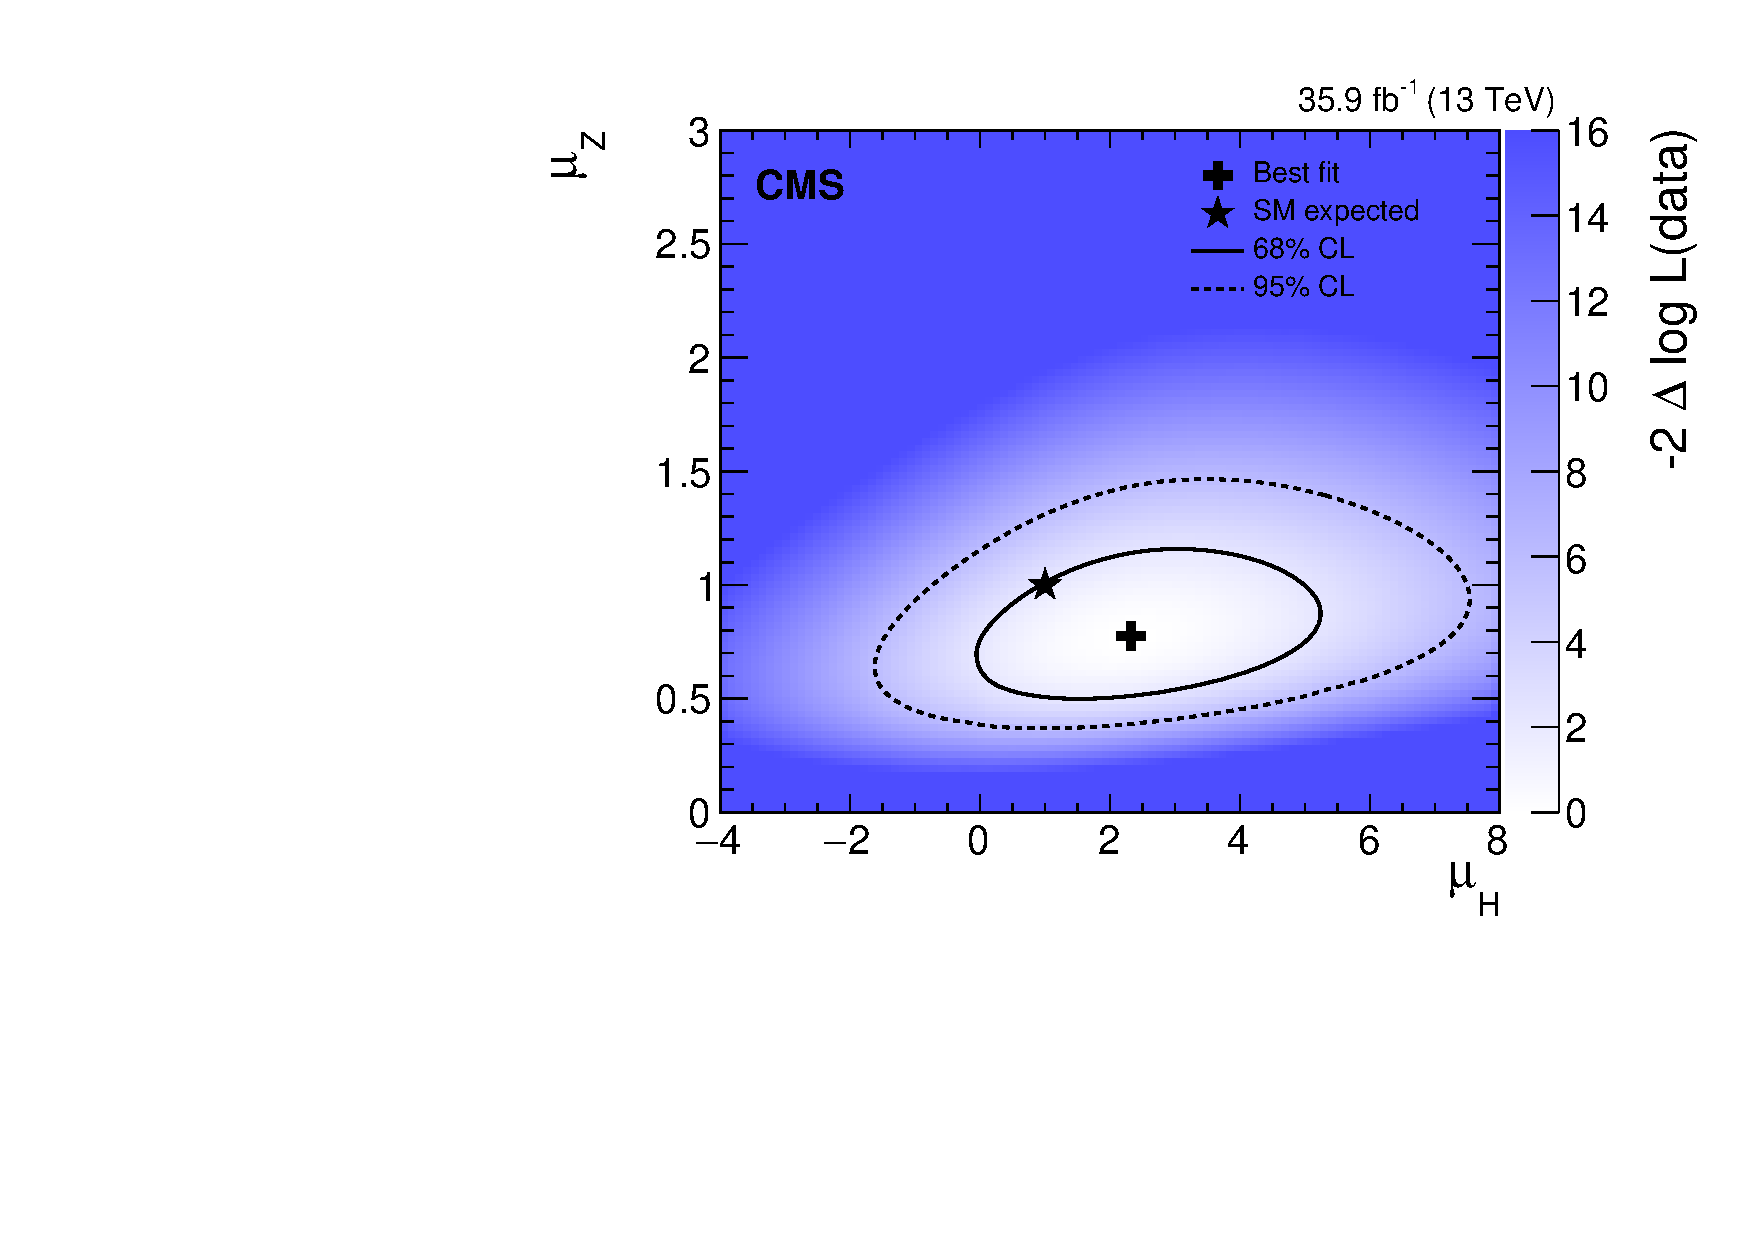
\includegraphics[width=0.49\linewidth]{img/inputs/hbb/signalstrengths.pdf}
    \caption{
        Resulting $\msd$ spectrum in the passing region from the $\hbb$ analysis~\cite{Sirunyan:2017dgc} (left), with the pink color-shaded area showing the contribution from $\ggh\to\bbbar$, and the signal strengths of the $\zboson\to\bbbar$ and $\hbb$ channels (right).
        % 
        Both taken from Ref.~\cite{Sirunyan:2017dgc}
        }
    \label{fig:hbbresults}
  \end{center}
\end{figure}



% ____________________________________________________________________________
\subsection{Modifications to the inputs for the combination}

With respect to the analyses performed in Refs.~\cite{Sirunyan:2018kta,Sirunyan:2017exp,Sirunyan:2017dgc}, a few adaptations were made in order to facilitate the combination of differential cross sections performed in Section~\ref{sec:diffxs}.
% 
For $\hgg$, the signal contributions were split into contributions from only $\ggh$ and other production modes.
% 
Additionally, the binning of the differential variables was modified slightly: The $\pth$ spectrum contains an additional bin, $\pth>600$\GeV, and an additional bin boundary at $\absy = 1.2$ is included in the $\absy$ spectrum.
% 
For $\hzz$, the binning was adapted in order to conform with those from the $\hgg$ analysis, and the branching fractions of the two $\zboson$ bosons to the various lepton configurations are fixed to their SM values, as opposed to floating branching fractions in the individual analysis.

The individual $\hbb$ analysis does not contain a differential measurement.
% 
It was created for the purpose of the combination, by splitting the signal into two $\pt$ bins, the first with $350\le\pt<600$\GeV and the second an overflow bin with $\pt\ge600$\GeV, which aligns with the binning of the other channels.
% 
The binning at the reconstructed level is set to $400\le\pt<600$ and $\pt\ge600$\GeV, and necessitates a reevaluation of the polynomial parametrization of $R_\text{p/f}$.


In order to combine differential measurements, all inputs must apply a common generator-level binning, which corresponds to the finest generator-level binning of the $\hgg$ channel.
% 
However, as the $\hzz$ and $\hbb$ channels often lack statistical precision in such a fine binning scheme, the results of these decay channels individually are sometimes reported in a coarser binning.
% 
This coarser binning is in these cases also the reconstruction-level binning of the respective channel.
% 
The reconstruction-level binning for each of the four differential variables is given in Tables~\ref{tab:binningpth}--\ref{tab:binningptjet}.



\begin{table*}[htb]
    \centering
    \topcaption{
        The reconstruction-level binning for $\pth$ for the $\hgg$, $\hzz$, and $\hbb$ channels.
        This binning coincides with the binning of the unfolded cross sections in which the individual results are reported.
        }
    \label{tab:binningpth}
    \tabletextwidth{
    \setlength{\tabcolsep}{5pt}
    \begin{tabular}{lccccccccc}
    Channel & \multicolumn{9}{l}{$\pth$ binning (GeV)} \\[\tablelineskip]
    \hline
    $\hgg$
        & [0, 15)    & [15, 30)   & [30, 45)   & [45, 80)        & [80, 120)
        & [120, 200) & [200, 350) & [350, 600) & [600, $\infty$)
        \\
    $\hzz$
        & [0, 15) & [15, 30)
        & \multicolumn{2}{l}{[30,  80)}
        & \multicolumn{2}{l}{[80,  200)}
        & \multicolumn{3}{l}{[200, $\infty$)}
        \\
    $\hbb$
        & \multicolumn{7}{@{{}}c@{{}}}{None} & [350, 600) & [600, $\infty$)
        \\
    \end{tabular}
    }
    \end{table*}

\begin{table}[htb]
    \centering
    \topcaption{
        The binning for $\njets$ for the $\hgg$ and the $\hzz$ channels.
        This binning coincides with the binning of the unfolded cross sections in which the individual results are reported.
        }
    \label{tab:binningnjets}
    \begin{tabular}{lccccc}
    Channel & \multicolumn{5}{l}{$\njets$ binning} \\[\tablelineskip]
    \hline
    $\hgg$ & 0 & 1 & 2 & 3 & $\ge$4 \\
    $\hzz$ & 0 & 1 & 2 & \multicolumn{2}{l}{$\ge$3} \\
    \end{tabular}
    \end{table}

\begin{table*}[htb]
    \centering
    \topcaption{
        The binning for $\absy$ for the $\hgg$ and the $\hzz$ channels.
        This binning coincides with the binning of the unfolded cross sections in which the individual results are reported.
        }
    \label{tab:binningabsy}
    \begin{tabular}{lcccccc}
    Channel & \multicolumn{6}{l}{$\absy$ binning} \\[\tablelineskip]
    \hline
    $\hgg$ & [0.0, 0.15) & [0.15, 0.30) & [0.30, 0.60) & [0.60, 0.90) & [0.90, 1.20) & [1.20, 2.50] \\
    $\hzz$ & [0.0, 0.15) & [0.15, 0.30) & [0.30, 0.60) & [0.60, 0.90) & [0.90, 1.20) & [1.20, 2.50] \\
    \end{tabular}
    \end{table*}

\begin{table*}[h!]
    \centering
    \topcaption{
        The binning for $\ptjet$ for the $\hgg$ and the $\hzz$ channels.
        This binning coincides with the binning of the unfolded cross sections in which the individual results are reported.
        }
    \label{tab:binningptjet}
    \begin{tabular}{lcccccc}
    Channel & \multicolumn{6}{l}{$\ptjet$ binning (GeV)} \\[\tablelineskip]
    \hline
    $\hgg$ & [0, 30) & [30, 55) & [55, 95) & [95, 120) & [120, 200) & [200, $\infty$) \\
    $\hzz$ & [0, 30) & [30, 55) & [55, 95) & \multicolumn{3}{l}{ [95, $\infty$) } \\
    \end{tabular}
    \end{table*}









% For $\hbb$ the signal is split into two $\pt$ bins at the generator level:
% the first with $350\le\pt<600$\GeV and the second an overflow bin with $\pt\ge600$\GeV, which aligns with the binning of the other channels.
% At the reconstruction level two bins are employed, with $400\le\pt<600$ and $\pt\ge600$\GeV, which is a slight modification with respect to the binning used in Ref.~\cite{CMS_AN_2016-366}.
% The redefinition of the reconstructed $\pt$ categories necessitates a reevaluation of the background model, which is performed using the same procedure as in the original analysis.




% \subsection{Paper text}

% For all the analyses used as input to the combination ($\hgg$~\cite{Sirunyan:2018kta}, $\hzztofourl$~\cite{CMS_AN_2016-442}, and $\hbb$~\cite{CMS_AN_2016-366}), the data set corresponds to an integrated luminosity of $35.9\fbinv$ recorded by the CMS experiment in 2016.
% The $\hbb$ decay channel is only included in the combination of the $\pth$ spectra, improving the measurements at the higher end of the distribution ($\pth > 350$\GeV) where the data from the $\hgg$ and $\hzz$ decay channels are limited.
% All analyses provide the parametrization of the folding matrix $M_{ji}^{k}$ (which is the probability for an event in generator-level bin $i$ to be reconstructed in bin $j$ and category $k$) in terms of a common generator-level binning, that is used for the combined spectra.
% Given the limited statistical precision in the individual channels, the results of the $\hzz$ and $\hbb$ channels individually are reported for a coarser binning, which is provided in Tables~\ref{tab:binningpth}--\ref{tab:binningptjet} for each of the observables.
% This binning coincides with the binning at the reconstruction level.


% The SM prediction for the differential cross sections is simulated with $\MGvATNLO$ v2.2.2~\cite{Alwall:2014hca} for each of the four dominant Higgs boson production modes: gluon-gluon fusion (\ggh), vector boson fusion, associated production with a $\wboson$/$\zboson$ boson, and associated production with a top quark-antiquark pair.
% A contribution from Higgs boson production in association with bottom quarks is not simulated, but included assuming its acceptance is equal to that from Higgs boson production via gluon fusion.
% The matrix element calculation includes the emission of up to two additional partons and is performed at NLO accuracy in perturbative quantum chromodynamics (QCD).
% Events are interfaced to \PYTHIA8.205~\cite{Sjostrand:2014zea} for parton showering and hadronization with the CUETP8M1~\cite{Skands:1695787} underlying event tune.
% The matrix element calculation is matched to the parton shower following the prescription in Ref.~\cite{Frederix:2012ps}.
% A weight depending on $\pth$ and $\njets$ is applied to simulated $\ggh$ events to match the predictions from the {\textsc{nnlops}} program~\cite{Hamilton:2012np, Kardos:2014dua}, as discussed in Ref.~\cite{Sirunyan:2018koj}.
% The set of parton distribution functions used in all simulations is NNPDF3.0~\cite{Ball:2014uwa}.
% The hadronic jets are clustered from the particle-flow candidates~\cite{Sirunyan:2017ulk} in the case of data and simulation, and from stable particles excluding neutrinos in the case of generated events, using the anti-$\kt$ clustering algorithm~\cite{Cacciari:2008gp} with a distance parameter of $0.4$.
% The measurements are reported in terms of kinematic observables defined before the decay of the Higgs boson, i.e. at the generator level.


% Each of the analyses used as input to the combination corresponds to a different fiducial phase space definition and applies a different event categorization.
% In the case of the $\hgg$ analysis, the fiducial phase space is defined by requiring the ratio of the leading (subleading) photon $\pt$ to the diphoton mass to be greater than $1/3$ ($1/4$).
% In addition, for each photon candidate the scalar sum of the generator-level $\pt$ of stable particles contained in a cone of radius $\Delta R=0.3$ around the candidate is required to be less than 10\GeV, where $\Delta R = \sqrt{\smash[b]{(\Delta\eta)^2+(\Delta\phi)^2}}$ is the angular separation between particles and $\Delta\phi$ is the azimuthal angle between two particles in radians.
% The selected photon pairs are categorized according to their estimated relative invariant mass resolution~\cite{Sirunyan:2018kta}.

% In the case of the $\hzz$ analysis, the 4-lepton mass is required to be greater than 70\GeV, the leading $\zboson$ boson candidate invariant mass must be greater than 40\GeV, and leptons must be separated in angular space by at least $\Delta R > 0.02$.
% Furthermore, at least two leptons must each have a $\pt>10$\GeV and at least one a $\pt > 20$\GeV.
% The selected events are categorized according to their lepton configuration in the final state (4 electrons, 4 muons, or 2 electrons and 2 muons).

% In the case of the $\hbb$ analysis, the analysis strategy requires the presence of a single anti-$\kt$ jet with a distance parameter of $0.8$, $\pt>450\,$GeV, and $\abs{\eta}<2.5$.
% For this analysis, the data is not unfolded to a fiducial phase space.
% Soft and wide-angle radiation is removed using the soft-drop grooming algorithm~\cite{Dasgupta:2013ihk,Larkoski:2014wba}.
% The jet mass after application of the soft-drop algorithm, $\msd$, peaks close to the Higgs boson mass in the case of signal events.
% To avoid finite-cone effects and the nonperturbative regime of the $\msd$ calculation, events are selected based on the dimensionless mass scale variable for QCD jets defined as $\rho=\log\left(\msd^2/\pt^2\right)$~\cite{Dasgupta:2013ihk}, which relates the jet $\pt$ to the jet mass.
% Events with isolated electrons, muons, or \taulepton leptons with $\pt>10$\GeV and $\abs{\eta}<2.5$ are vetoed in order to reduce the background from SM electroweak processes, and events with a missing transverse momentum greater than $140$\GeV are vetoed in order to reduce the background from top quark-antiquark pair production.
% Additionally, a selection criterion is applied based on the compatibility of the single anti-$\kt$ jet with having a two-prong substructure~\cite{Dolen:2016kst,Moult:2016cvt,Larkoski:2013eya,Thaler:2010tr}.
% Events are categorized according to their likelihood of consisting of two $\bquark$ quarks, which is computed using the double-$\bquark$ tagger algorithm~\cite{Sirunyan:2017ezt}.


% Minor modifications are applied to the individual analyses in Refs.~\cite{Sirunyan:2018kta,CMS_AN_2016-442,CMS_AN_2016-366} to provide the inputs used for the combination of differential observables.
% For $\hgg$, an additional bin, $\pth>600$\GeV, is included in the $\pth$ spectrum.
% For $\hzz$, the binning is modified for multiple kinematic observables to align with the binning of the $\hgg$ analysis.
% Furthermore, the branching fractions of the two $\zboson$ bosons to the various lepton configurations are fixed to their SM values, whereas in Ref.~\cite{CMS_AN_2016-442} these are allowed to float.
% For $\hbb$ the signal is split into two $\pt$ bins at the generator level:
% the first with $350\le\pt<600$\GeV and the second an overflow bin with $\pt\ge600$\GeV, which aligns with the binning of the other channels.
% At the reconstruction level two bins are employed, with $400\le\pt<600$ and $\pt\ge600$\GeV, which is a slight modification with respect to the binning used in Ref.~\cite{CMS_AN_2016-366}.
% The redefinition of the reconstructed $\pt$ categories necessitates a reevaluation of the background model, which is performed using the same procedure as in the original analysis.
% For the purpose of the combination in this analysis, the fiducial measurements from the $\hgg$ and $\hzz$ channels are extrapolated to the inclusive phase space~\cite{Alwall:2014hca,Hamilton:2012np,Kardos:2014dua}.


% \begin{table*}[htb]
%     \centering
%     \topcaption{
%         The reconstruction-level binning for $\pth$ for the $\hgg$, $\hzz$, and $\hbb$ channels.
%         This binning coincides with the binning of the unfolded cross sections in which the individual results are reported.
%         }
%     \label{tab:binningpth}
%     \tabletextwidth{
%     \setlength{\tabcolsep}{5pt}
%     \begin{tabular}{lccccccccc}
%     Channel & \multicolumn{9}{l}{$\pth$ binning (GeV)} \\[\tablelineskip]
%     \hline
%     $\hgg$
%         & [0, 15)    & [15, 30)   & [30, 45)   & [45, 80)        & [80, 120)
%         & [120, 200) & [200, 350) & [350, 600) & [600, $\infty$)
%         \\
%     $\hzz$
%         & [0, 15) & [15, 30)
%         & \multicolumn{2}{l}{[30,  80)}
%         & \multicolumn{2}{l}{[80,  200)}
%         & \multicolumn{3}{l}{[200, $\infty$)}
%         \\
%     $\hbb$
%         & \multicolumn{7}{@{{}}c@{{}}}{None} & [350, 600) & [600, $\infty$)
%         \\
%     \end{tabular}
%     }
%     \end{table*}

% \begin{table}[htb]
%     \centering
%     \topcaption{
%         The binning for $\njets$ for the $\hgg$ and the $\hzz$ channels.
%         This binning coincides with the binning of the unfolded cross sections in which the individual results are reported.
%         }
%     \label{tab:binningnjets}
%     \begin{tabular}{lccccc}
%     Channel & \multicolumn{5}{l}{$\njets$ binning} \\[\tablelineskip]
%     \hline
%     $\hgg$ & 0 & 1 & 2 & 3 & $\ge$4 \\
%     $\hzz$ & 0 & 1 & 2 & \multicolumn{2}{l}{$\ge$3} \\
%     \end{tabular}
%     \end{table}

% \begin{table*}[htb]
%     \centering
%     \topcaption{
%         The binning for $\absy$ for the $\hgg$ and the $\hzz$ channels.
%         This binning coincides with the binning of the unfolded cross sections in which the individual results are reported.
%         }
%     \label{tab:binningabsy}
%     \begin{tabular}{lcccccc}
%     Channel & \multicolumn{6}{l}{$\absy$ binning} \\[\tablelineskip]
%     \hline
%     $\hgg$ & [0.0, 0.15) & [0.15, 0.30) & [0.30, 0.60) & [0.60, 0.90) & [0.90, 1.20) & [1.20, 2.50] \\
%     $\hzz$ & [0.0, 0.15) & [0.15, 0.30) & [0.30, 0.60) & [0.60, 0.90) & [0.90, 1.20) & [1.20, 2.50] \\
%     \end{tabular}
%     \end{table*}

% \begin{table*}[h!]
%     \centering
%     \topcaption{
%         The binning for $\ptjet$ for the $\hgg$ and the $\hzz$ channels.
%         This binning coincides with the binning of the unfolded cross sections in which the individual results are reported.
%         }
%     \label{tab:binningptjet}
%     \begin{tabular}{lcccccc}
%     Channel & \multicolumn{6}{l}{$\ptjet$ binning (GeV)} \\[\tablelineskip]
%     \hline
%     $\hgg$ & [0, 30) & [30, 55) & [55, 95) & [95, 120) & [120, 200) & [200, $\infty$) \\
%     $\hzz$ & [0, 30) & [30, 55) & [55, 95) & \multicolumn{3}{l}{ [95, $\infty$) } \\
%     \end{tabular}
%     \end{table*}

